%% ====================================================================
%%  Volatility Managed Portfolios, Master Project Report (v2)
%%  EDHEC Business School, Volatility Management Strategies
%%  Compiled with pdfLaTeX, natbib
%% ====================================================================
\documentclass[12pt, a4paper]{article}

%% Packages
\usepackage[T1]{fontenc}
\usepackage[utf8]{inputenc}
\usepackage[english]{babel}
\usepackage{times}

\usepackage[top=2.5cm, bottom=2.5cm, left=2.5cm, right=2.5cm]{geometry}
\usepackage{setspace}
\onehalfspacing

\usepackage{amsmath, amssymb, amsthm}

\usepackage{booktabs}
\usepackage{tabularx}
\usepackage{multirow}
\usepackage{array}
\usepackage{longtable}
\usepackage{siunitx}
\sisetup{group-separator={,}, group-minimum-digits=4}

\usepackage{graphicx}
\usepackage{float}
\usepackage{caption}
\usepackage{subcaption}
\captionsetup{font=small, labelfont=bf, margin=10pt}

\usepackage[dvipsnames]{xcolor}
\definecolor{edhec}{RGB}{0, 62, 126}

\usepackage[authoryear, round, sort]{natbib}

\usepackage[colorlinks=true,
            linkcolor=edhec,
            citecolor=edhec,
            urlcolor=edhec,
            pdftitle={Volatility Managed Portfolios},
            pdfauthor={EDHEC AMP}]{hyperref}

\usepackage{fancyhdr}
\setlength{\headheight}{14pt}
\pagestyle{fancy}
\fancyhf{}
\lhead{\small\textcolor{edhec}{\textit{Volatility Managed Portfolios}}}
\rhead{\small\textcolor{edhec}{\textit{EDHEC Business School}}}
\cfoot{\thepage}
\renewcommand{\headrulewidth}{0.4pt}

\usepackage{titlesec}
\titleformat{\section}{\large\bfseries\color{edhec}}{\thesection.}{0.8em}{}
\titleformat{\subsection}{\normalsize\bfseries}{\thesubsection.}{0.6em}{}
\titleformat{\subsubsection}{\normalsize\itshape}{\thesubsubsection.}{0.5em}{}

\usepackage{enumitem}
\usepackage{parskip}
\setlength{\parskip}{6pt}

%% Maths helpers
\newcommand{\E}{\mathbb{E}}
\newcommand{\stgt}{\sigma^{\mathrm{target}}}
\newcommand{\shat}{\hat{\sigma}}

%% ====================================================================
\begin{document}

\begin{titlepage}
\centering
\vspace*{2cm}
{\color{edhec}\rule{\linewidth}{1.5pt}}\\[0.4cm]
{\LARGE\bfseries\color{edhec} Volatility Managed Portfolios\\[0.3cm]
\large A Critical Assessment Across Five Asset Classes\\[0.2cm]
\normalsize January 2000 to December 2025}\\[0.4cm]
{\color{edhec}\rule{\linewidth}{1.5pt}}\\[1.5cm]
{\large\textit{Advanced Master Project}}\\[0.3cm]
{\large EDHEC Business School}\\[0.3cm]
{\large Volatility Management Strategies}\\[1.2cm]

{\normalsize Prepared by:}\\[0.3cm]
{\large \textbf{Camille Valat}}\\[0.1cm]
{\large \textbf{Alexandre Vincent}}\\[0.1cm]
{\large \textbf{Thomas Laumonier}}\\[0.4cm]
{\normalsize \textit{MSc in Financial Engineering}}\\[1.2cm]

{\normalsize Submitted to:}\\[0.2cm]
{\large\bfseries Prof.\ Nikos Tessaromatis}\\[0.2cm]
{\normalsize EDHEC Business School}\\[2cm]
{\normalsize April 2025}
\vfill
\end{titlepage}

%% ====================================================================
\begin{abstract}
\noindent
This report evaluates volatility-targeting strategies on five asset classes (US equities,
US long-term government bonds, commodities, the USD/JPY exchange rate, and the
Fama-French US momentum factor) over the period January 2000 to December 2025. We construct
four volatility forecasts at the monthly frequency: one-month realised volatility, six-month
realised volatility, a GJR-GARCH(1,1) with Student-$t$ errors, and an EGARCH(1,1). The
target volatility is computed with a strictly expanding window to avoid the look-ahead bias
discussed by \citet{Bongaerts2020}.

The point estimates of Sharpe ratio improvements are economically meaningful in three cases.
On the S\&P 500, GJR-GARCH lifts the Sharpe ratio from 0.658 to 0.785 and shortens the
longest drawdown from 52 to 40 months. On the momentum factor, the same model raises the
Sharpe ratio from 0.066 to 0.363 and cuts the worst drawdown duration from 205 to 73 months.
On USD/JPY, the improvement is smaller (Sharpe rising from 0.040 to 0.116) but consistently
positive across models.

Statistical inference, however, qualifies these results. Using the Jobson-Korkie test with
the Memmel (2003) correction and a circular block-bootstrap procedure (2,000 resamples,
six-month blocks), the only asset for which the Sharpe improvement is significant at the
5\% level is the momentum factor (bootstrap $p$-values between 0.003 and 0.015 across the
four models). The 95\% bootstrap confidence interval for the S\&P 500 GARCH improvement is
$[-0.10,\, +0.35]$, so the null of equal Sharpe cannot be rejected. Fama-French alpha
regressions corroborate this picture: alphas on the momentum factor are between 7.5\% and
8.7\% per year with $t$-statistics above 2.3, whereas the equity alpha falls below
significance once we control for the three-factor or five-factor model.

For commodities and US long-term bonds, the volatility-managed Sharpe ratio is lower
than that of buy and hold even at zero transaction cost; the strategy never breaks even at
any positive cost level. For the S\&P 500 and USD/JPY, the breakeven transaction cost lies
near 60 bps, comfortably above institutional execution costs. An equal-weighted multi-asset
portfolio of the five GJR-GARCH variants achieves a higher Sharpe ratio (0.673) than any
single-asset variant and reduces the maximum drawdown to 19.5\%, demonstrating that
volatility timing and cross-asset diversification stack rather than substitute.

The headline policy implication is therefore narrower than the prior literature suggests.
Statistically robust evidence in favour of volatility targeting exists only for the
momentum factor; for equities, the case is suggestive but not conclusive on Sharpe ratio
grounds.
\end{abstract}

\tableofcontents
\clearpage

%% ====================================================================
\section{Theory of Volatility-Targeting Strategies}
\label{sec:theory}
%% ====================================================================

\subsection{Conceptual Foundation}

Volatility-targeting strategies exploit a well-documented empirical regularity: although
expected returns are notoriously difficult to forecast, conditional return volatility is
predictable at both short and medium horizons \citep{Andersen2003}. This predictability
creates an asymmetric opportunity. An investor who reduces exposure before high-volatility
regimes, when the variance-risk premium is elevated and crash risk is greatest, should
obtain superior risk-adjusted returns without relying on any return-forecasting ability.

The foundational modern treatment is \citet{Moreira2017}, who show that scaling a
portfolio weight inversely with its predicted variance generates portfolios with higher
Sharpe ratios and substantially reduced maximum drawdowns across US equity factors.
\citet{Harvey2018} extend the result to a broader cross-section of asset classes and
document consistent improvements in risk-adjusted returns under institutional-quality
transaction cost assumptions. The asset management industry has adopted volatility
targeting widely; assets under management in related strategies (risk-parity funds,
variable annuities, systematic trend-following) exceed one trillion US dollars.

A separate strand of the literature is more sceptical. \citet{Liu2019} examine the same
US equity factors as \citet{Moreira2017} and argue that the published Sharpe improvements
largely vanish once the look-ahead bias in the target volatility is removed and once the
Sharpe differences are tested formally. Their study motivates our use of an expanding
window for the target volatility (Section~\ref{sec:lookahead}) and our explicit testing of
Sharpe ratio differences (Section~\ref{sec:sr_tests}).

\subsection{Formal Framework}

At the beginning of month $t$, the weight on asset $i$ is set so that the portfolio's
forecasted volatility equals a target level:
\begin{equation}
  w_{i,t} \;=\; \frac{\stgt}{\shat_{i,t}},
  \label{eq:weight}
\end{equation}
where $w_{i,t}$ is the monthly weight on asset $i$, $\stgt$ is the long-run target
volatility level (expressed in annualised standard deviation units), and $\shat_{i,t}$
denotes the conditional one-period-ahead volatility forecast for asset $i$, formed at the
end of month $t-1$ and expressed in the same annualised units.

The realised return of the managed portfolio in month $t$ is then
\begin{equation}
  r_{i,t}^{\mathrm{vm}} \;=\;
  \begin{cases}
    r_{f,t} + w_{i,t}\bigl(r_{i,t} - r_{f,t}\bigr) & \text{long-only assets,}\\
    w_{i,t}\, r_{i,t} & \text{long-short self-financing assets,}
  \end{cases}
  \label{eq:returns}
\end{equation}
where $r_{i,t}$ is the realised monthly total return of asset $i$ and $r_{f,t}$ is the
monthly risk-free rate, both expressed as decimal returns. When the predicted volatility
falls below target, the strategy levers up. When predicted volatility rises, the strategy
scales down, limiting drawdown risk. We follow \citet{Bongaerts2020} in setting the
scaling constant $k = 1$ in the more general formula $w_{i,t} = (\stgt/\shat_{i,t})\cdot k$.
Any choice $k\neq 1$ that brings the realised volatility of the managed portfolio exactly
onto its target uses information from the entire sample and is therefore not
implementable in real time. Section~\ref{sec:diag_k} reports the ex-post implied values of
$k$ as a diagnostic. A maximum leverage constraint $w_{i,t} \leq w_{\max}$ prevents
unbounded leverage in extremely low-volatility regimes.

\subsection{Look-Ahead Bias in the Target Volatility}
\label{sec:lookahead}

The full-sample standard deviation
$\sigma^{\mathrm{full}} = \mathrm{std}(r_1, r_2, \ldots, r_T)$,
used as the target volatility in \citet{Moreira2017} and \citet{Harvey2018}, introduces a
look-ahead bias because the value of the target at any date $t$ depends on observations
from $t+1$ to $T$. The strategy is then calibrated, by construction, to the realised
long-run volatility of the underlying asset, and its realised volatility will be close to
the target by construction.

Following \citet{Bongaerts2020} (Section~III.A), we eliminate this bias by replacing the
full-sample standard deviation by an expanding-window estimator:
\begin{equation}
  \stgt_t \;=\; \mathrm{std}\!\left(r_1, r_2, \ldots, r_{\tau_{t-1}}\right),
  \label{eq:target}
\end{equation}
where $\tau_{t-1}$ denotes the last trading day of month $t-1$ and the standard deviation
is computed on the daily simple returns up to that date. Under this definition,
$\stgt_t$ is observable at time $t$ without any future information. As $t$ approaches the
sample end, $\stgt_t$ converges to the full-sample standard deviation, but at any
intermediate date it is strictly backward-looking. We impose a minimum 48-month estimation
window before computing portfolio weights, to ensure that the initial values of
$\stgt_t$ and the GARCH parameter estimates are statistically reliable.

Section~\ref{sec:diag_lookahead} reports an empirical comparison between
Equation~\eqref{eq:target} and the look-ahead-biased full-sample alternative. The size of
the bias is asset-specific and, surprisingly, modest in our sample; nonetheless, only the
bias-free specification is consistent with real-time deployment.

\subsection{Theoretical Mechanisms and Conditions for Profitability}

Table~\ref{tab:theory} summarises the main theoretical channels through which volatility
targeting is expected to generate value.

\begin{table}[H]
  \centering
  \caption{Theoretical Mechanisms Supporting Volatility-Targeting Strategies}
  \label{tab:theory}
  \small
  \begin{tabularx}{\textwidth}{lXl}
    \toprule
    \textbf{Mechanism} & \textbf{Description} & \textbf{Reference} \\
    \midrule
    Variance-risk premium
      & High volatility states coincide with elevated variance-risk premia; de-risking
        avoids paying the premium while benefiting from low-volatility upside
      & \citet{Moreira2017} \\[4pt]
    Inverse volatility to return relationship
      & Conditional Sharpe ratios are systematically lower in high-volatility regimes
        across most asset classes
      & \citet{Harvey2018} \\[4pt]
    Drawdown mitigation
      & Automatic de-risking before crises reduces left-tail exposure and limits
        momentum crashes
      & \citet{Bongaerts2020} \\[4pt]
    No return-timing required
      & The strategy exploits only volatility predictability, which is robust, without
        requiring expected-return forecasts
      & \citet{Harvey2018} \\[4pt]
    Reduced negative skewness
      & Scaling down before volatility spikes truncates the left tail, improving the
        higher moments of the return distribution
      & \citet{Moreira2017} \\
    \bottomrule
  \end{tabularx}
\end{table}

The strategy is expected to add value when three conditions hold jointly. First,
volatility must be sufficiently predictable, that is, the Mincer-Zarnowitz $R^2$ of the
forecast versus the subsequent realised volatility must be materially positive. Second,
the conditional Sharpe ratio must be decreasing in volatility, so that risk premia do not
adequately compensate for spikes in risk. Third, transaction costs must be small enough
relative to the frequency and magnitude of weight changes. If volatility is essentially
unpredictable, or if the conditional Sharpe ratio is positively correlated with
volatility (as is plausible for government bonds during flight-to-quality episodes), the
strategy can destroy value.

\subsection{Critiques of the Literature}

\citet{Liu2019} identify three concerns about the published evidence. First, the
look-ahead bias in $\stgt$ inflates the reported Sharpe improvements (we revisit this
empirically in Section~\ref{sec:diag_lookahead}). Second, the performance is concentrated
around the 2008 financial crisis and may not extend out of sample. Third, the strategy
operates primarily as a crisis-avoidance mechanism rather than as a source of structural
alpha. Their finding that Sharpe ratio improvements lose statistical significance after
bias correction motivates two design choices in this report: a bias-free implementation
of the target volatility (Section~\ref{sec:lookahead}) and explicit Sharpe ratio
significance tests on every strategy-asset pair (Section~\ref{sec:sr_tests}).


%% ====================================================================
\section{Data}
\label{sec:data}
%% ====================================================================

\subsection{Asset Universe and Sources}

The study covers five assets representing distinct risk premia and asset classes. All data
were sourced from Bloomberg and Kenneth French's data library, spanning January 2000 to
December 2025 (6,542 daily observations, 264 monthly observations after the 48-month
warm-up period). The Fama-French factors used in Section~\ref{sec:perf_ff} were taken from
Kenneth French's data library at the daily frequency and aggregated to monthly returns by
compounding.

\begin{table}[H]
  \centering
  \caption{Asset Universe: Description and Sources}
  \label{tab:data_desc}
  \small
  \begin{tabularx}{\textwidth}{llXl}
    \toprule
    \textbf{Ticker} & \textbf{Asset} & \textbf{Description} & \textbf{Return Type} \\
    \midrule
    SPXT     & S\&P 500 TR           & S\&P 500 Total Return Index; dividends reinvested
                                     & Total Return \\
    LT09TRUU & US LT Bonds TR        & Bloomberg US Long Treasury Total Return Index;
                                       coupons reinvested
                                     & Total Return \\
    BCOMCOT  & Bloomberg Commodities & Bloomberg Commodity Total Return Index; roll yield
                                       and collateral return included
                                     & Total Return \\
    USDJPY   & USD/JPY               & US Dollar / Japanese Yen spot exchange rate
                                     & Price Return \\
    MOM      & US Momentum Factor    & Fama-French US momentum factor (long winners, short
                                       losers); sourced from Kenneth French
                                     & Long-Short (decimal) \\
    USGG3M   & 3-Month US T-Bill     & Annualised yield; used as the risk-free rate proxy
                                     & Yield \\
    \midrule
    MKT-RF   & Market factor         & Excess return on the value-weighted US market
                                       portfolio over the risk-free rate
                                     & Factor return \\
    SMB      & Size factor           & Small Minus Big return spread
                                     & Factor return \\
    HML      & Value factor          & High Minus Low return spread on book-to-market
                                     & Factor return \\
    RMW      & Profitability factor  & Robust Minus Weak return spread on operating
                                       profitability
                                     & Factor return \\
    CMA      & Investment factor     & Conservative Minus Aggressive return spread on
                                       asset growth
                                     & Factor return \\
    \bottomrule
  \end{tabularx}
\end{table}

\noindent\textbf{Return construction.}
Daily simple returns are computed as $r_t = P_t/P_{t-1} - 1$ for the four index or
exchange-rate series, where $P_t$ is the price at the close of day $t$. The momentum
factor is expressed as a daily percentage return by Kenneth French and converted to a
decimal by dividing by 100. The risk-free rate is compounded daily as
$r_{f,t} = (1 + y_t/100)^{1/252} - 1$, where $y_t$ is the annualised three-month T-bill
yield. Monthly returns are the cumulative product of daily returns within each calendar
month.

\noindent\textbf{Total return consideration.}
We use total return indices for equities, bonds, and commodities, which include
dividends, coupon income, and roll plus collateral return respectively. This choice is
essential for a fair comparison: the volatility-targeting weight applies to the complete
economic return, not merely to the price change. For USD/JPY (a currency rate), only the
price return is available; the carry differential is not explicitly modelled and the
treatment of FX exposure is therefore conservative.

\subsection{Descriptive Statistics}

Table~\ref{tab:desc_stats} reports annualised descriptive statistics for the full sample.

\begin{table}[H]
  \centering
  \caption{Descriptive Statistics: January 2000 to December 2025}
  \label{tab:desc_stats}
  \small
  \begin{tabular}{lccccc}
    \toprule
    \textbf{Asset} & \textbf{Ann. Return} & \textbf{Ann. Volatility} & \textbf{Sharpe}
                   & \textbf{Skewness} & \textbf{Exc. Kurtosis} \\
    \midrule
    S\&P 500 TR              & 7.8\%  & 19.4\% &  0.31 & $-$0.35 & 10.63 \\
    US LT Bonds TR           & 4.2\%  &  6.6\% &  0.37 & $-$0.01 &  2.64 \\
    Bloomberg Commodities    & 6.6\%  & 34.0\% &  0.14 & $-$0.69 &  9.38 \\
    USD/JPY                  & 1.3\%  &  9.7\% & $-$0.04 & $-$0.13 & 4.27 \\
    US Momentum Factor       & 3.8\%  & 16.7\% &  0.12 & $-$0.71 &  6.54 \\
    \bottomrule
  \end{tabular}
\end{table}

\noindent
Three features deserve attention. First, commodities exhibit the highest volatility
(34.0\%) but the lowest Sharpe ratio among directional assets, reflecting the difficulty
of earning a structural risk premium on commodity beta. Second, all assets display
negative skewness and positive excess kurtosis, consistent with the fat tails commonly
documented on financial return distributions and confirming the relevance of tail-risk
management. Third, the momentum factor, despite being self-financing, exhibits pronounced
negative skewness ($-0.71$) and excess kurtosis (6.54), reflecting the momentum crash
phenomenon studied by \citet{Moreira2017}.

\subsection{Correlation Structure}

As shown in Figure~\ref{fig:data_overview}, cross-asset return correlations are uniformly
near zero (every pair has $|\rho| \leq 0.02$). This near-orthogonality justifies treating
each asset independently in a single-asset volatility-targeting framework and implies that
multi-asset diversification benefits are largely independent of any intra-asset
volatility-timing benefit. The single-asset strategies studied below can therefore serve
as building blocks in a multi-asset portfolio without introducing spurious cross-asset
dependencies. We exploit this property explicitly in Section~\ref{sec:multi_asset}.

\begin{figure}[H]
  \centering
  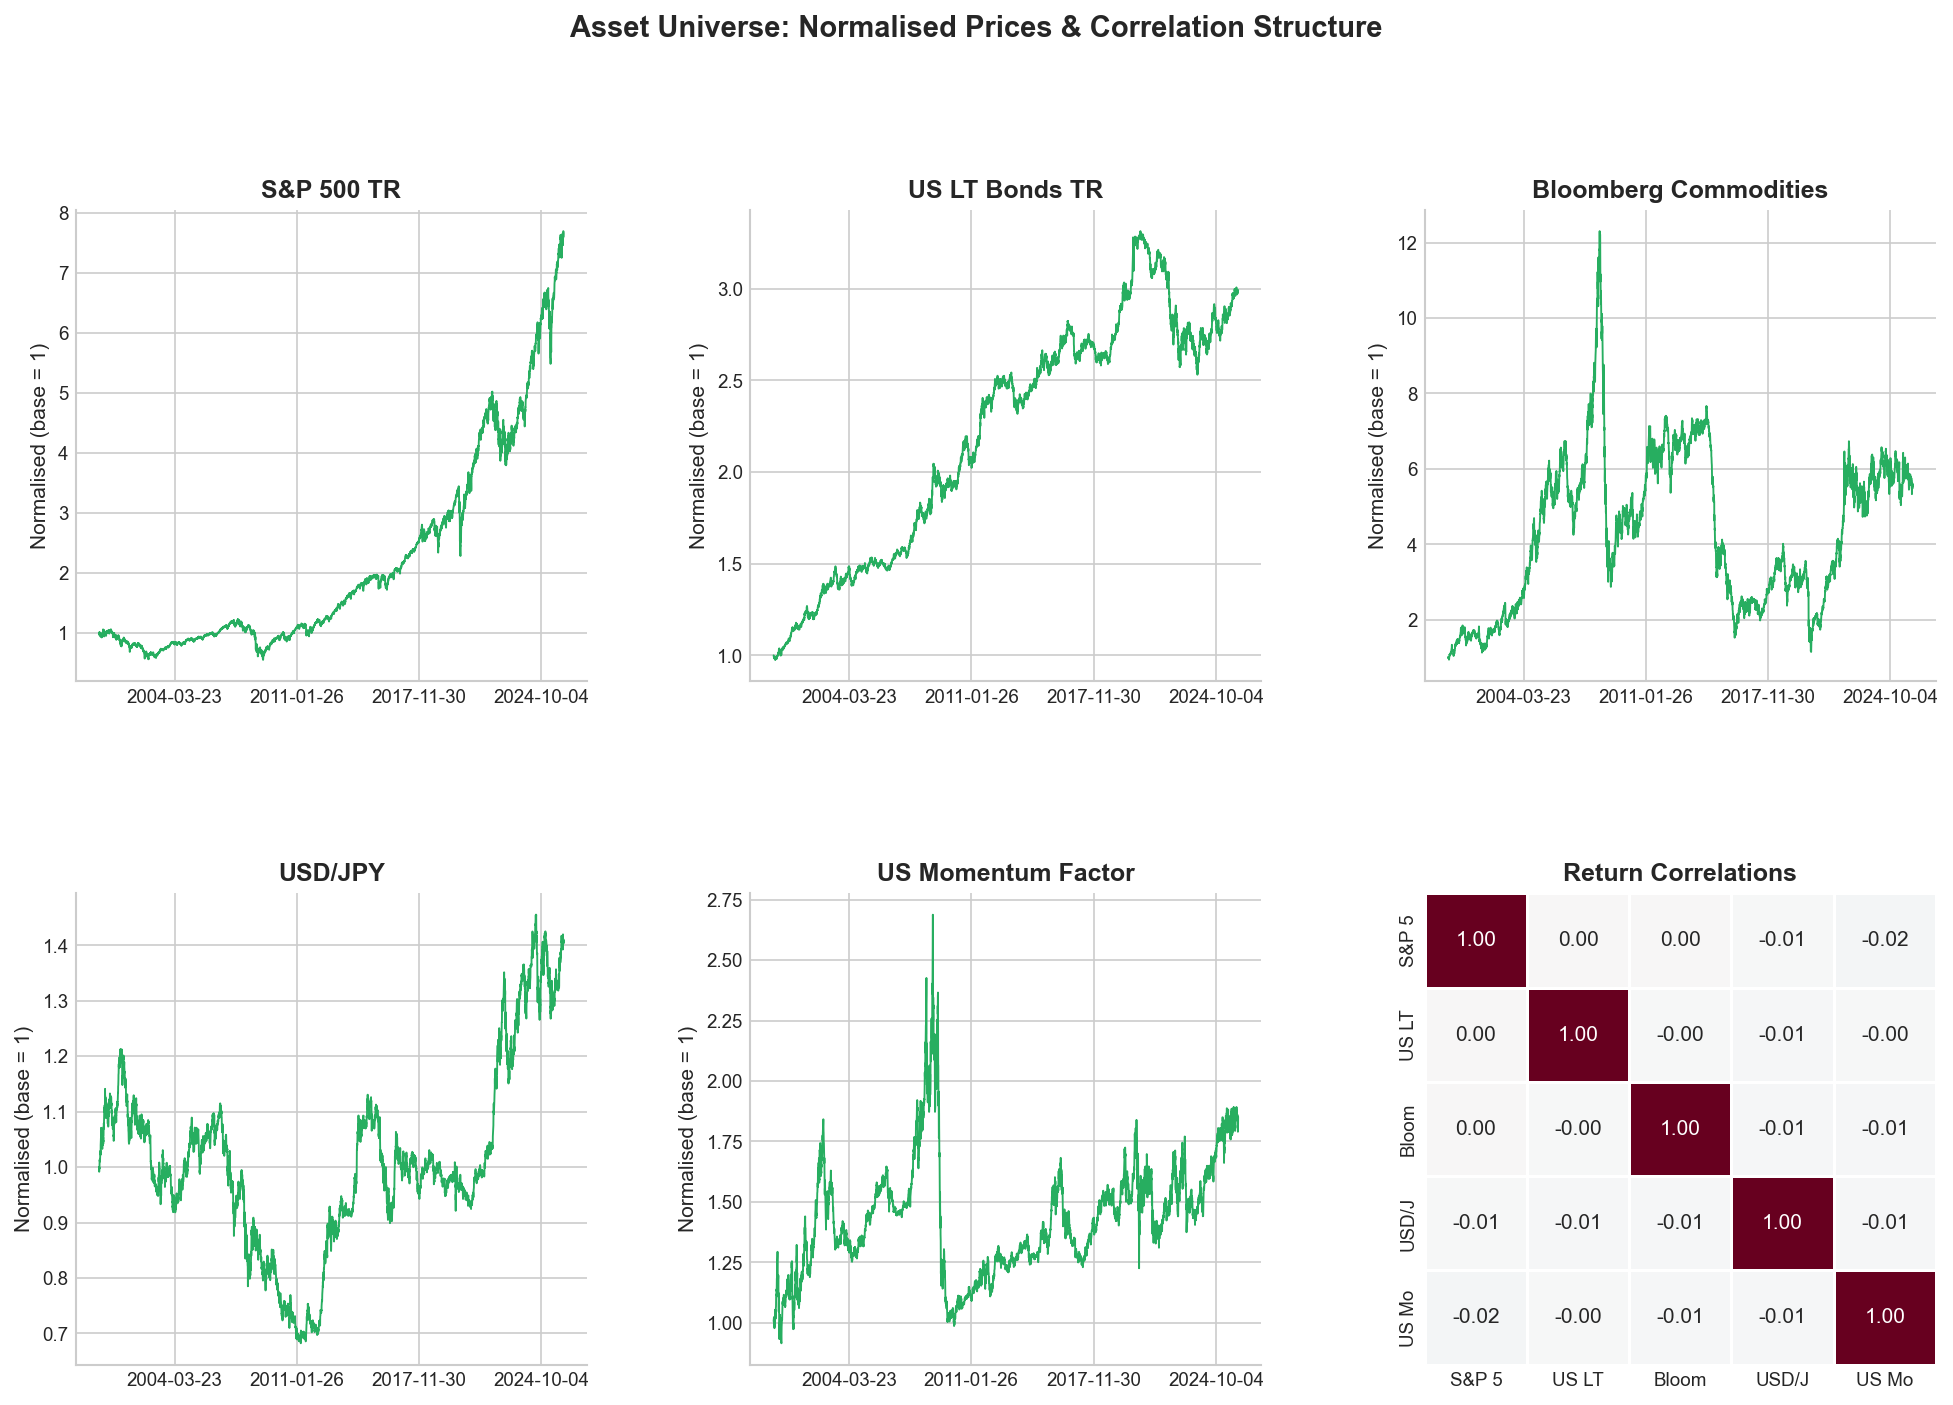
\includegraphics[width=0.95\textwidth]{fig_01_data_overview.png}
  \caption{Asset Universe: Normalised Prices (base = 1) and Pairwise Return Correlations
           (January 2000 to December 2025). All cross-asset correlations are below 0.02
           in absolute value. The five return trajectories differ markedly: the S\&P 500
           grows by a factor of 7.6 over the sample while the Bloomberg Commodity Index
           peaks in 2008 and subsequently declines from approximately 12$\times$ to
           approximately 6$\times$.}
  \label{fig:data_overview}
\end{figure}


%% ====================================================================
\section{Methodology}
\label{sec:methodology}
%% ====================================================================

\subsection{Implementation Choices}
\label{sec:implementation}

Table~\ref{tab:implementation} summarises the key design choices made in this study and
their academic justifications.

\begin{table}[H]
  \centering
  \caption{Implementation Choices for the Volatility-Targeting Strategy}
  \label{tab:implementation}
  \small
  \begin{tabularx}{\textwidth}{lXX}
    \toprule
    \textbf{Parameter} & \textbf{Value or Rule} & \textbf{Rationale} \\
    \midrule
    Target volatility $\stgt$ & Expanding-window standard deviation of daily returns up
                                to end of month $t-1$
      & Avoids look-ahead bias \citep{Bongaerts2020} \\
    Scaling constant $k$ & 1 (no ex-post rescaling) & Implementable in real time \\
    Leverage cap & $w_{\max} = 2.0$ (baseline) & Realistic institutional constraint \\
    Transaction cost & 10 basis points one-way (baseline) & Consistent with institutional
                                                            estimates \citep{Frazzini2018} \\
    Cost application & $r_t^{\mathrm{net}} = r_t^{\mathrm{vm}} - |\Delta w_t| \cdot c$
      & One-way cost on each weight change \\
    Return frequency & Monthly (compounded from daily) & Avoids monthly-return bias \\
    Minimum estimation window & 48 months ($\approx 4$ years) & Ensures reliable GARCH
                                                                estimation \\
    \bottomrule
  \end{tabularx}
\end{table}

\subsection{Volatility Forecasting Models}

We implement four forecasting models, all using strictly backward-looking expanding-window
data at the point of each monthly weight computation.

\paragraph{One-month realised volatility.}
The one-month realised volatility is the equal-weighted standard deviation of daily returns
in month $t-1$, annualised by $\sqrt{252}$:
\begin{equation}
  \shat^{\mathrm{RV1M}}_{i,t} \;=\;
  \sqrt{\frac{252}{n_{t-1}} \sum_{s \in t-1} r_{i,s}^2 },
\end{equation}
where $n_{t-1}$ is the number of trading days in month $t-1$ and $r_{i,s}$ is the daily
return of asset $i$ on day $s$ within that month. This is the benchmark of
\citet{Moreira2017}. Its parsimony makes it a natural baseline, but it reacts sharply to
individual monthly outliers and can overestimate volatility for several months after a
crisis.

\paragraph{Six-month realised volatility.}
The six-month realised volatility uses daily returns over months $t-6$ to $t-1$:
\begin{equation}
  \shat^{\mathrm{RV6M}}_{i,t} \;=\;
  \sqrt{ \frac{252}{N_t} \sum_{s=\tau_{t-6}}^{\tau_{t-1}} r_{i,s}^2 },
\end{equation}
where $N_t$ is the number of trading days between $\tau_{t-6}$ and $\tau_{t-1}$. The
longer window reduces noise at the cost of slower reaction to regime shifts. The implicit
equal weighting over six months also means that crisis observations are diluted over six
months rather than one, which reduces post-crisis overestimation at the expense of
underestimation at the onset of a spike.

\paragraph{GJR-GARCH(1,1) with Student-$t$ errors.}
The GJR-GARCH model of \citet{Glosten1993} captures the leverage effect, that is, the
asymmetric response of equity volatility to negative returns documented in equity markets.
We estimate it on daily returns scaled by 100, with the specification
\begin{align}
  r_{i,t} &= \sigma_{i,t}\,\varepsilon_{i,t},
  \qquad \varepsilon_{i,t} \sim t_\nu, \\
  \sigma_{i,t}^2 &= \omega + \alpha\, r_{i,t-1}^2
                   + \gamma\, r_{i,t-1}^2\,\mathbf{1}[r_{i,t-1}<0]
                   + \beta\,\sigma_{i,t-1}^2,
\end{align}
where $\sigma_{i,t}$ is the conditional standard deviation, $\varepsilon_{i,t}$ is a
Student-$t$ innovation with $\nu$ degrees of freedom, and $\omega > 0$, $\alpha \geq 0$,
$\beta \geq 0$, $\gamma \geq 0$ are the GARCH parameters. The indicator
$\mathbf{1}[r_{i,t-1}<0]$ equals one when the previous daily return was negative; the
parameter $\gamma > 0$ controls the asymmetric impact of negative shocks on future
variance. Persistence of shocks is governed by $\alpha + \gamma/2 + \beta < 1$. The
monthly forecast is the average 21-day-ahead variance under the GARCH recursion:
$\shat^{\mathrm{GARCH}}_{i,t} = \sqrt{252 \cdot \overline{V}_{21}}$, with $\overline{V}_{21}$
the simple average of the 21 daily variance forecasts. Student-$t$ errors are used to
accommodate the fat-tailed nature of daily returns evident in
Table~\ref{tab:desc_stats}. The model is re-estimated each month on all data available at
the end of the month (expanding window) by quasi-maximum likelihood.

\paragraph{EGARCH(1,1).}
The EGARCH model of \citet{Nelson1991} operates on log-variance, which eliminates
non-negativity constraints and allows the sign of the return shock to affect the
conditional variance independently of its magnitude:
\begin{equation}
  \log\sigma_{i,t}^2 \;=\; \omega + \beta\,\log\sigma_{i,t-1}^2
                            + \alpha\,\frac{|r_{i,t-1}|}{\sigma_{i,t-1}}
                            + \gamma\,\frac{r_{i,t-1}}{\sigma_{i,t-1}}.
\end{equation}
Here $\sigma_{i,t}^2$ is the conditional variance and $\omega$, $\alpha$, $\beta$,
$\gamma$ are the EGARCH parameters. The log specification ensures $\sigma_{i,t}^2 > 0$
for all parameter values, providing greater numerical stability for assets like USD/JPY
with near-zero mean returns. EGARCH serves as a robustness check for GJR-GARCH;
differences in portfolio performance between the two GARCH variants provide indirect
evidence of the importance of the leverage specification.

\subsection{Forecast Evaluation Methodology}

\paragraph{Error metrics.}
We report Root Mean Squared Error (RMSE), Mean Absolute Error (MAE), and Mean Absolute
Percentage Error (MAPE) against the subsequent month's realised volatility, computed as
the equal-weighted daily standard deviation over the next 21 trading days.

\paragraph{Mincer-Zarnowitz regression.}
The regression of \citet{Mincer1969} assesses forecast unbiasedness and efficiency:
\begin{equation}
  \sigma_{i,t+1}^{\mathrm{realised}} \;=\; \alpha + \beta\,\shat_{i,t} + u_{t+1},
  \label{eq:mz}
\end{equation}
where $\sigma_{i,t+1}^{\mathrm{realised}}$ is the realised annualised volatility of asset
$i$ in month $t+1$, $\shat_{i,t}$ is the model forecast formed at the end of month $t$,
$\alpha$ and $\beta$ are regression coefficients, and $u_{t+1}$ is a residual. An unbiased
and efficient forecast satisfies $\alpha = 0$ and $\beta = 1$ jointly; rejection of this
joint hypothesis by an $F$-test indicates forecast bias. The $R^2$ of the regression
measures the fraction of realised volatility variation explained by the forecast.

\paragraph{Diebold-Mariano test.}
Pairwise forecast accuracy comparisons use the \citet{DM1995} test with squared-error
loss and a Newey-West variance adjustment (one lag):
\begin{equation}
  d_t \;=\; e_{1,t}^2 - e_{2,t}^2,
  \qquad
  \mathrm{DM} \;=\; \frac{\bar{d}}{\sqrt{\widehat{\mathrm{LRV}}(d)/T}}
                  \;\xrightarrow{d}\; \mathcal{N}(0,1),
\end{equation}
where $e_{1,t}$ and $e_{2,t}$ are the forecast errors of models 1 and 2 at date $t$,
$\bar{d}$ is the sample mean of $d_t$, $\widehat{\mathrm{LRV}}(d)$ is the
Newey-West long-run variance estimator of $d_t$, and $T$ is the sample size. A negative
DM statistic (positive $\bar{d}$) implies that model 1 is less accurate than model 2.

\subsection{Performance Evaluation}

Performance statistics are computed at the monthly frequency on compounded returns.
Table~\ref{tab:stats_def} defines each statistic.

\begin{table}[H]
  \centering
  \caption{Performance Statistics: Definitions}
  \label{tab:stats_def}
  \small
  \begin{tabularx}{\textwidth}{lX}
    \toprule
    \textbf{Statistic} & \textbf{Definition} \\
    \midrule
    Annualised return       & Geometrically compounded: $(1+\bar{r})^{12/T}-1$, with
                              $\bar{r}$ the arithmetic mean monthly return and $T$ the
                              number of months. \\
    Annualised volatility   & Standard deviation of monthly returns multiplied by
                              $\sqrt{12}$. \\
    Sharpe ratio            & Mean monthly excess return over the three-month T-bill,
                              annualised by multiplying by 12, divided by the annualised
                              volatility. \\
    Sortino ratio           & Annualised excess mean return divided by the annualised
                              downside deviation (computed only on negative excess
                              returns). \\
    Maximum drawdown        & The largest peak-to-trough decline in cumulative wealth:
                              $\min_t \{ (C_t - \max_{s\leq t} C_s)\,/\,\max_{s\leq t} C_s \}$,
                              where $C_t$ is the cumulative wealth at month $t$. \\
    Drawdown duration       & The longest consecutive number of months in which the
                              cumulative wealth lies below its prior peak. \\
    Recovery time           & The number of months between the trough of the worst
                              drawdown and the recovery of the prior peak; reported as
                              ``not recovered'' if the prior peak has not been reached
                              by the end of the sample. \\
    Expected shortfall (5\%)& Mean monthly return conditional on the return being below
                              the 5\% empirical quantile:
                              $\E[r_t \mid r_t \leq q_{5\%}]$. \\
    Annualised turnover     & Mean monthly absolute weight change multiplied by 12:
                              $12 \cdot \E[|w_t - w_{t-1}|]$. \\
    CAPM Alpha and Beta     & Intercept (annualised) and slope of an OLS regression of
                              the monthly excess return on the own-asset Buy and Hold
                              excess return. \\
    Information ratio       & Annualised mean active return divided by annualised tracking
                              error against the own-asset Buy and Hold. \\
    Appraisal ratio         & CAPM alpha divided by the annualised standard deviation of
                              the regression residuals. \\
    \bottomrule
  \end{tabularx}
\end{table}

\noindent
The CAPM alpha reported in Section~\ref{sec:performance} uses each asset's own Buy and
Hold strategy as the benchmark, so it measures the abnormal return of the
volatility-managed variant relative to the unmanaged variant of the same asset. This
single-factor specification is informative for a within-asset comparison but does not
control for systematic risk factors such as market, size, value, profitability or
investment exposures. Section~\ref{sec:perf_ff} therefore augments the analysis with
Fama-French three-factor and five-factor regressions on the S\&P 500 and on the momentum
factor, the two assets for which a multi-factor specification is most natural.

\subsection{Sharpe Ratio Significance Tests}
\label{sec:sr_tests}

To assess whether observed Sharpe ratio differences are statistically meaningful, we
implement two complementary tests on every pair of (volatility-managed strategy versus
Buy and Hold) and on the GJR-GARCH versus EGARCH pair.

\paragraph{Jobson-Korkie test with Memmel correction.}
The test of \citet{JobsonKorkie1981}, corrected by \citet{Memmel2003}, evaluates the null
hypothesis $H_0$: $\mathrm{SR}_1 = \mathrm{SR}_2$ under the assumption of independent,
identically distributed and jointly normal returns. The test statistic is
\begin{equation}
  z \;=\;
  \frac{\widehat{\mathrm{SR}}_1 - \widehat{\mathrm{SR}}_2}
       {\sqrt{\hat\theta / T}},
  \qquad
  \hat\theta \;=\;
  2(1 - \hat\rho)
  + \tfrac{1}{2}\bigl(\widehat{\mathrm{SR}}_1^2 + \widehat{\mathrm{SR}}_2^2
                       - 2\,\widehat{\mathrm{SR}}_1\,\widehat{\mathrm{SR}}_2\,\hat\rho^2\bigr),
\end{equation}
where $\widehat{\mathrm{SR}}_1$ and $\widehat{\mathrm{SR}}_2$ are the sample monthly
Sharpe ratios of the two strategies, $\hat\rho$ is the sample correlation of their excess
returns, and $T$ is the number of monthly observations. Under $H_0$, $z$ converges to a
standard normal distribution. The Memmel correction relative to the original
Jobson-Korkie formula corrects an upward bias in the variance estimator that becomes
material in small samples.

\paragraph{Block bootstrap test.}
Monthly returns of volatility-managed strategies exhibit autocorrelation and fat tails
that violate the assumptions underlying the Jobson-Korkie test. We therefore complement
it with a circular block bootstrap in the spirit of \citet{LedoitWolf2008}: with
$B = 2{,}000$ resamples and block length of six months, we generate bootstrap
distributions of the Sharpe ratio difference $\widehat{\mathrm{SR}}_1^* - \widehat{\mathrm{SR}}_2^*$.
The two-sided $p$-value for $H_0$ is computed from the bootstrap distribution centred at
the observed difference, and a 95\% percentile confidence interval is reported. Confidence
intervals that contain zero indicate that the null of equal Sharpe ratio cannot be
rejected at the 5\% level.

\subsection{Fama-French Alpha Regressions}
\label{sec:meth_ff}

For the S\&P 500 and the momentum factor, we run additional alpha regressions on the
Fama-French three-factor and five-factor models:
\begin{equation}
  r_{i,t}^{\mathrm{exc}} \;=\;
  \alpha_i
  + \beta_{i}^{\mathrm{MKT}} \mathrm{MKT}_t
  + \beta_{i}^{\mathrm{SMB}} \mathrm{SMB}_t
  + \beta_{i}^{\mathrm{HML}} \mathrm{HML}_t
  \;[+\,\beta_{i}^{\mathrm{RMW}} \mathrm{RMW}_t + \beta_{i}^{\mathrm{CMA}} \mathrm{CMA}_t]
  + u_{i,t},
  \label{eq:ff}
\end{equation}
where $r_{i,t}^{\mathrm{exc}}$ is the monthly excess return of strategy $i$ on asset $i$,
$\mathrm{MKT}_t$, $\mathrm{SMB}_t$, $\mathrm{HML}_t$, $\mathrm{RMW}_t$, $\mathrm{CMA}_t$
are the Fama-French market, size, value, profitability and investment factors
respectively, $\beta_i^{\bullet}$ are the corresponding factor loadings, $\alpha_i$ is the
annualised abnormal return, and $u_{i,t}$ is a residual. The bracketed terms are present
in the five-factor specification only. Inference uses Newey-West heteroskedasticity and
autocorrelation consistent (HAC) standard errors with six lags.

For the momentum factor, the Fama-French momentum factor is itself the asset, so we
exclude the momentum factor from the right-hand side of Equation~\eqref{eq:ff}. The
resulting alpha measures the value added by volatility-managing the momentum factor on
top of static exposure to the equity-style factors.

We do not run Fama-French regressions on the other three assets (US long-term bonds,
commodities and USD/JPY) because the Fama-French factors are designed to span the
equity-return generating process, not the bond, commodity or FX cross-section. A proper
multi-factor risk model for these assets would involve term and default factors, commodity
carry and momentum factors, and FX carry and value factors. We acknowledge this as a
limitation and rely on the within-asset CAPM alpha defined in Table~\ref{tab:stats_def}.


%% ====================================================================
\section{Volatility Forecast Evaluation}
\label{sec:forecast}
%% ====================================================================

\subsection{Error Metrics and Mincer-Zarnowitz Results}

Table~\ref{tab:mz} reports the full set of forecast evaluation statistics for the five
assets. Figure~\ref{fig:vol_forecasts} shows the time-series of forecasts versus realised
volatility, and Figure~\ref{fig:forecast_bar} provides a bar-chart comparison of RMSE,
MAPE and correlation.

\begin{table}[H]
  \centering
  \caption{Volatility Forecast Evaluation: RMSE, MAPE, Correlation, and Mincer-Zarnowitz
           Regression by Asset and Model}
  \label{tab:mz}
  \footnotesize
  \begin{tabular}{llccccccc}
    \toprule
    \textbf{Asset} & \textbf{Model}
      & \textbf{RMSE} & \textbf{MAE} & \textbf{MAPE}
      & \textbf{Corr.} & {$\hat{\alpha}$} & {$\hat{\beta}$} & {$R^2$} \\
    \midrule
    \multirow{4}{*}{S\&P 500 TR}
      & RV 1M        & 0.0894 & 0.0545 & 0.3678 & 0.6479 &  0.0534 & 0.6481 & 0.4198 \\
      & RV 6M        & 0.1027 & 0.0612 & 0.4414 & 0.4785 &  0.0595 & 0.5592 & 0.2289 \\
      & GJR-GARCH    & \bfseries 0.0737 & 0.0490 & 0.3743 & \bfseries 0.7374 &  0.0089 & 0.8754 & \bfseries 0.5438 \\
      & EGARCH       & 0.0751 & 0.0486 & 0.3706 & 0.7132 & {$-$0.0172} & 1.0718 & 0.5087 \\
    \midrule
    \multirow{4}{*}{US LT Bonds TR}
      & RV 1M        & 0.0214 & 0.0139 & 0.2344 & 0.6047 & 0.0237 & 0.6059 & 0.3656 \\
      & RV 6M        & 0.0198 & 0.0139 & 0.2477 & 0.6234 & 0.0133 & 0.7433 & 0.3886 \\
      & GJR-GARCH    & 0.0191 & 0.0129 & 0.2330 & 0.6487 & 0.0078 & 0.8197 & 0.4209 \\
      & EGARCH       & \bfseries 0.0183 & 0.0126 & 0.2258 & \bfseries 0.6704 & 0.0034 & 0.8946 & \bfseries 0.4494 \\
    \midrule
    \multirow{4}{*}{Bloomberg Comm.}
      & RV 1M        & 0.1271 & 0.0849 & 0.2868 & 0.6369 & 0.1080 & 0.6373 & 0.4057 \\
      & RV 6M        & 0.1419 & 0.0933 & 0.3287 & 0.4811 & 0.1125 & 0.5834 & 0.2314 \\
      & GJR-GARCH    & 0.1233 & 0.0878 & 0.3260 & 0.6204 & 0.0434 & 0.7791 & 0.3848 \\
      & EGARCH       & \bfseries 0.1160 & 0.0834 & 0.3067 & \bfseries 0.6493 & 0.0004 & 0.9275 & \bfseries 0.4216 \\
    \midrule
    \multirow{4}{*}{USD/JPY}
      & RV 1M        & 0.0374 & 0.0269 & 0.3123 & 0.5139 & 0.0424 & 0.5139 & 0.2641 \\
      & RV 6M        & 0.0354 & 0.0268 & 0.3301 & 0.4812 & 0.0289 & 0.6285 & 0.2316 \\
      & GJR-GARCH    & 0.0332 & 0.0257 & 0.3371 & 0.5463 & 0.0123 & 0.7874 & 0.2984 \\
      & EGARCH       & \bfseries 0.0329 & 0.0250 & 0.3249 & \bfseries 0.5318 & 0.0049 & 0.8789 & \bfseries 0.2829 \\
    \midrule
    \multirow{4}{*}{US Momentum}
      & RV 1M        & 0.0543 & 0.0375 & 0.3033 & 0.8102 & 0.0250 & 0.8103 & 0.6564 \\
      & RV 6M        & 0.0656 & 0.0433 & 0.3844 & 0.7069 & 0.0250 & 0.7673 & 0.4997 \\
      & GJR-GARCH    & \bfseries 0.0519 & 0.0360 & 0.3060 & \bfseries 0.8213 & 0.0105 & 0.9027 & \bfseries 0.6745 \\
      & EGARCH       & 0.0519 & 0.0361 & 0.3073 & 0.8173 & 0.0118 & 0.8897 & 0.6680 \\
    \bottomrule
  \end{tabular}
  \begin{minipage}{\textwidth}
    \vspace{2pt}
    \footnotesize\textit{Notes.} Best performer per asset highlighted in bold. The
    Mincer-Zarnowitz $F$-test of the joint hypothesis $\hat{\alpha} = 0$ and
    $\hat{\beta} = 1$ rejects unbiasedness ($p < 0.05$) for RV 1M and RV 6M on every asset,
    and for GJR-GARCH on every asset except the S\&P 500, where EGARCH is the only
    model that fails to reject ($p = 0.241$). Corr.\ refers to the Pearson correlation
    with realised monthly volatility.
  \end{minipage}
\end{table}

\begin{figure}[H]
  \centering
  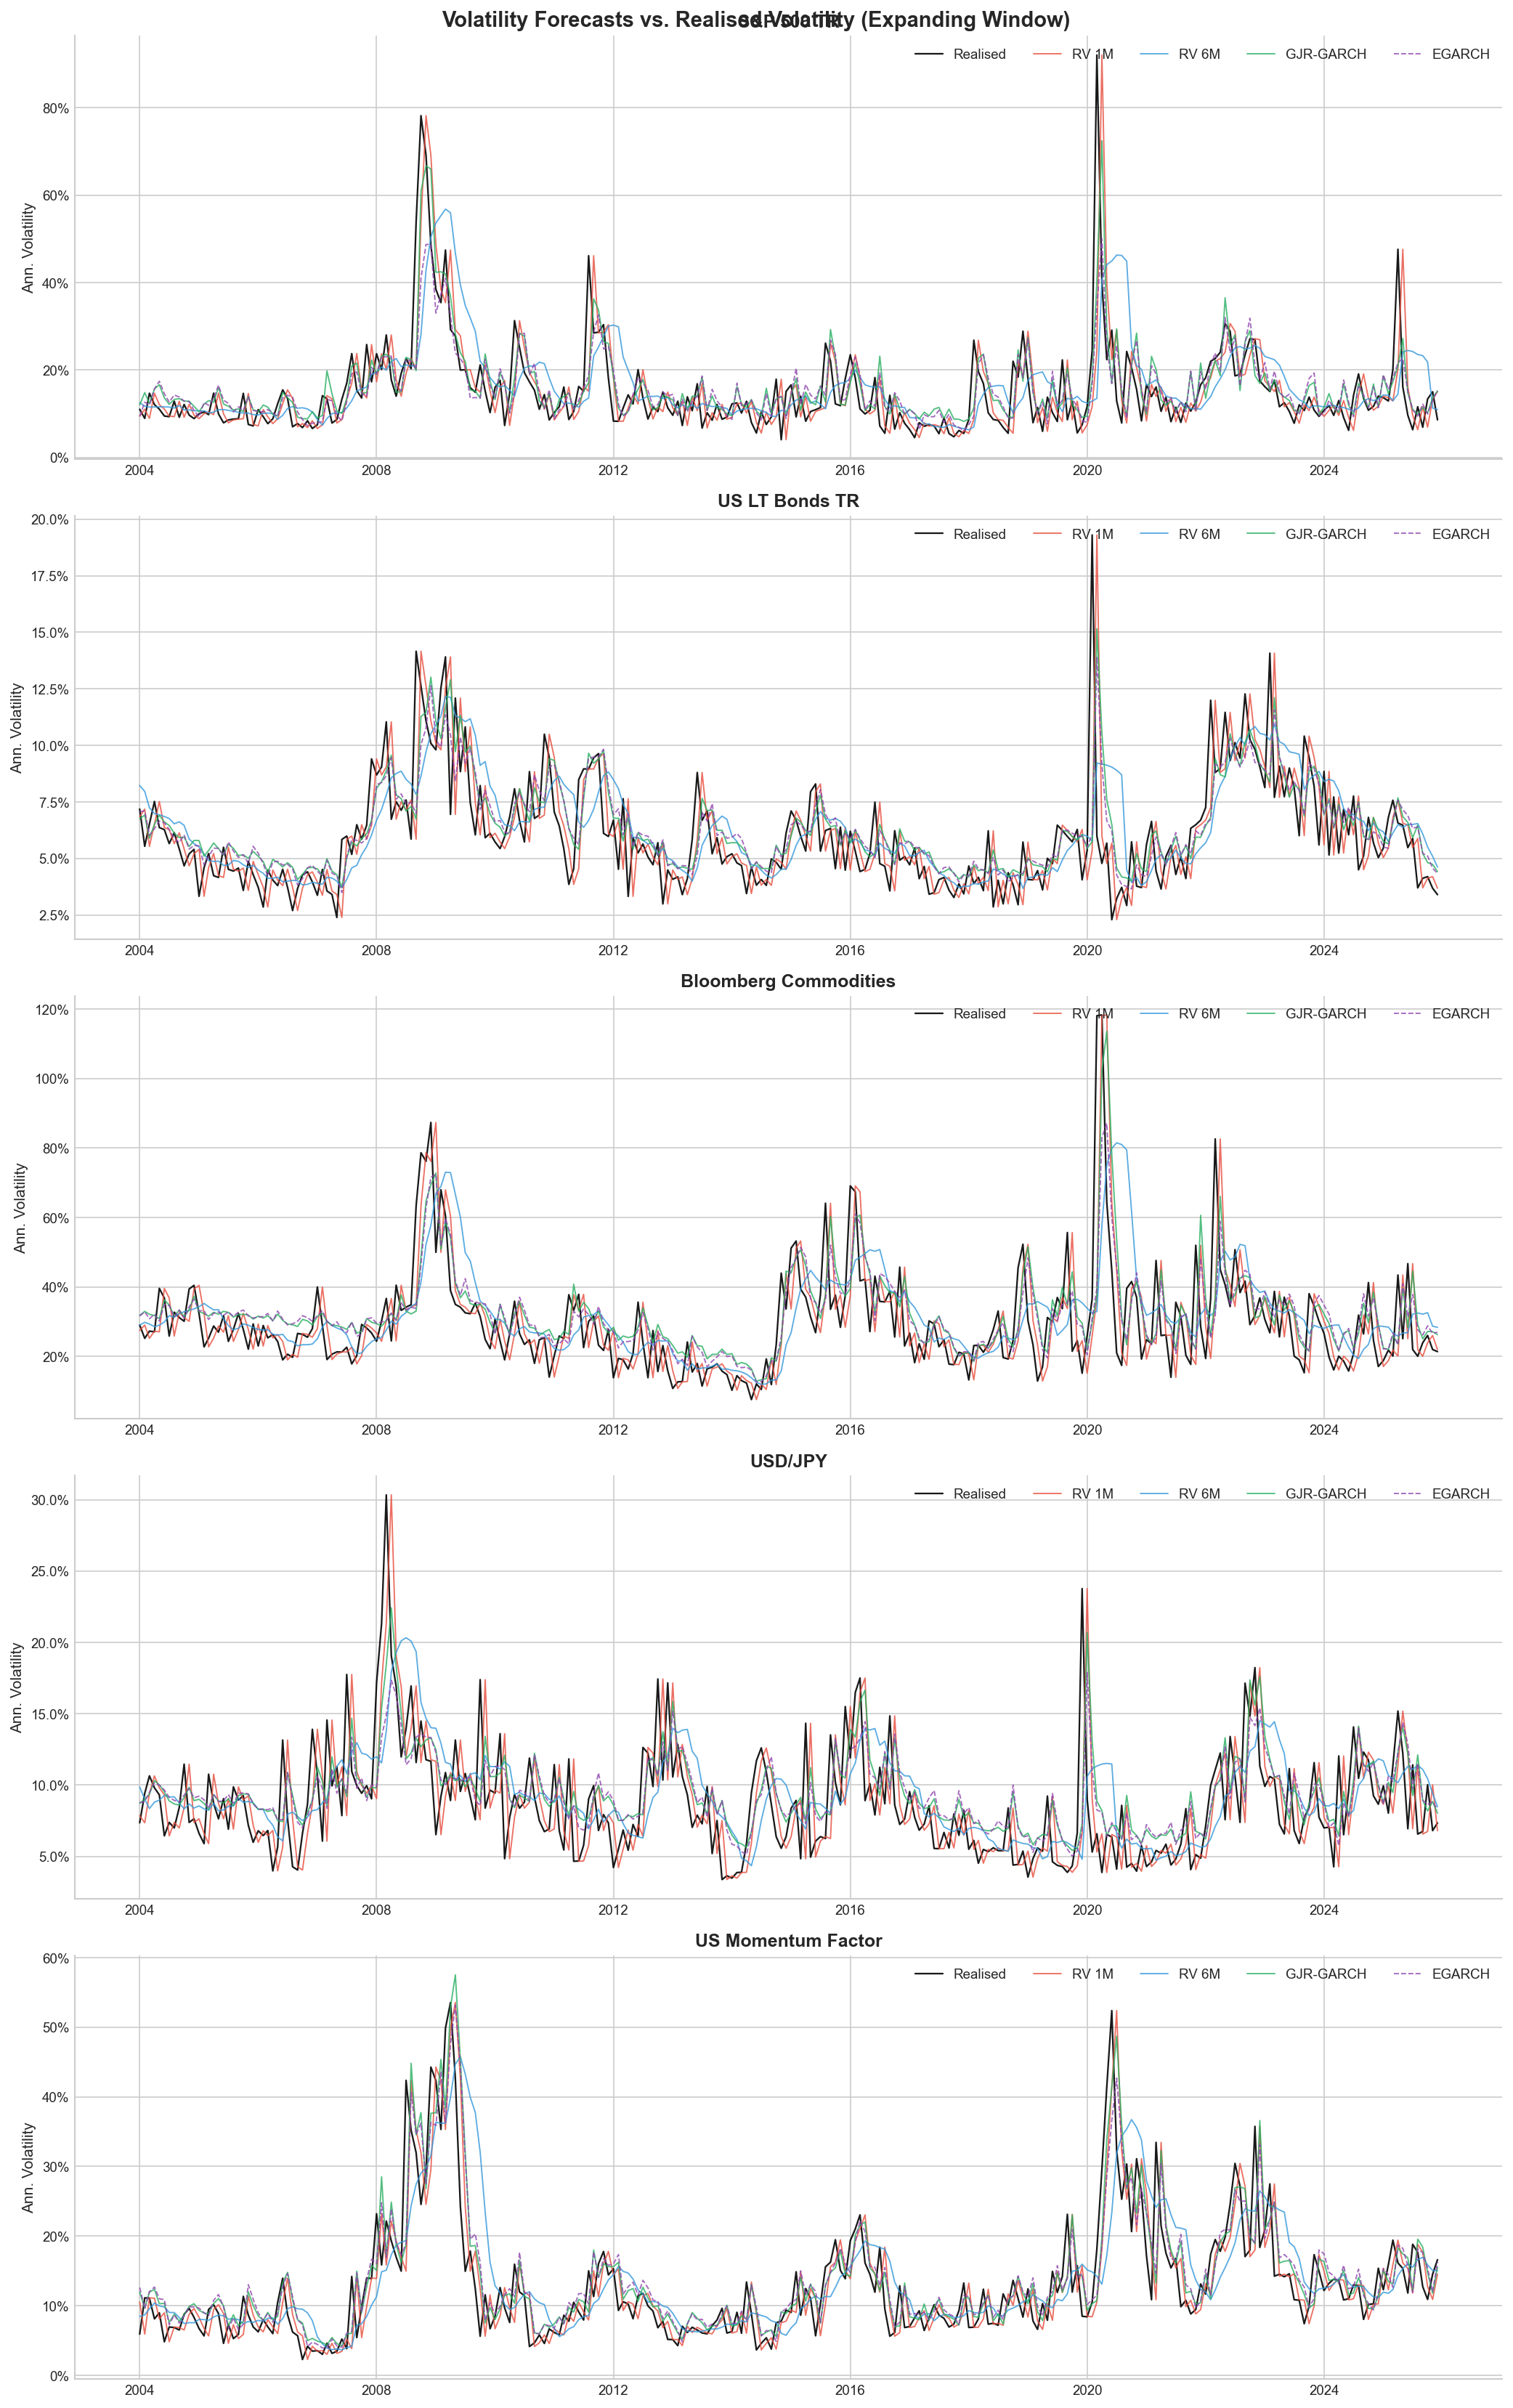
\includegraphics[width=0.88\textwidth]{fig_02_vol_forecasts.png}
  \caption{Volatility Forecasts versus Realised Volatility (expanding window), all five
           assets. GJR-GARCH and EGARCH react more smoothly to regime shifts and closely
           track realised volatility during the 2008 financial crisis and the COVID-19
           shock of 2020. RV 1M spikes sharply following high-volatility months, a
           ``volatility echo'' effect, while RV 6M systematically underestimates at the
           onset of volatility spikes.}
  \label{fig:vol_forecasts}
\end{figure}

\begin{figure}[H]
  \centering
  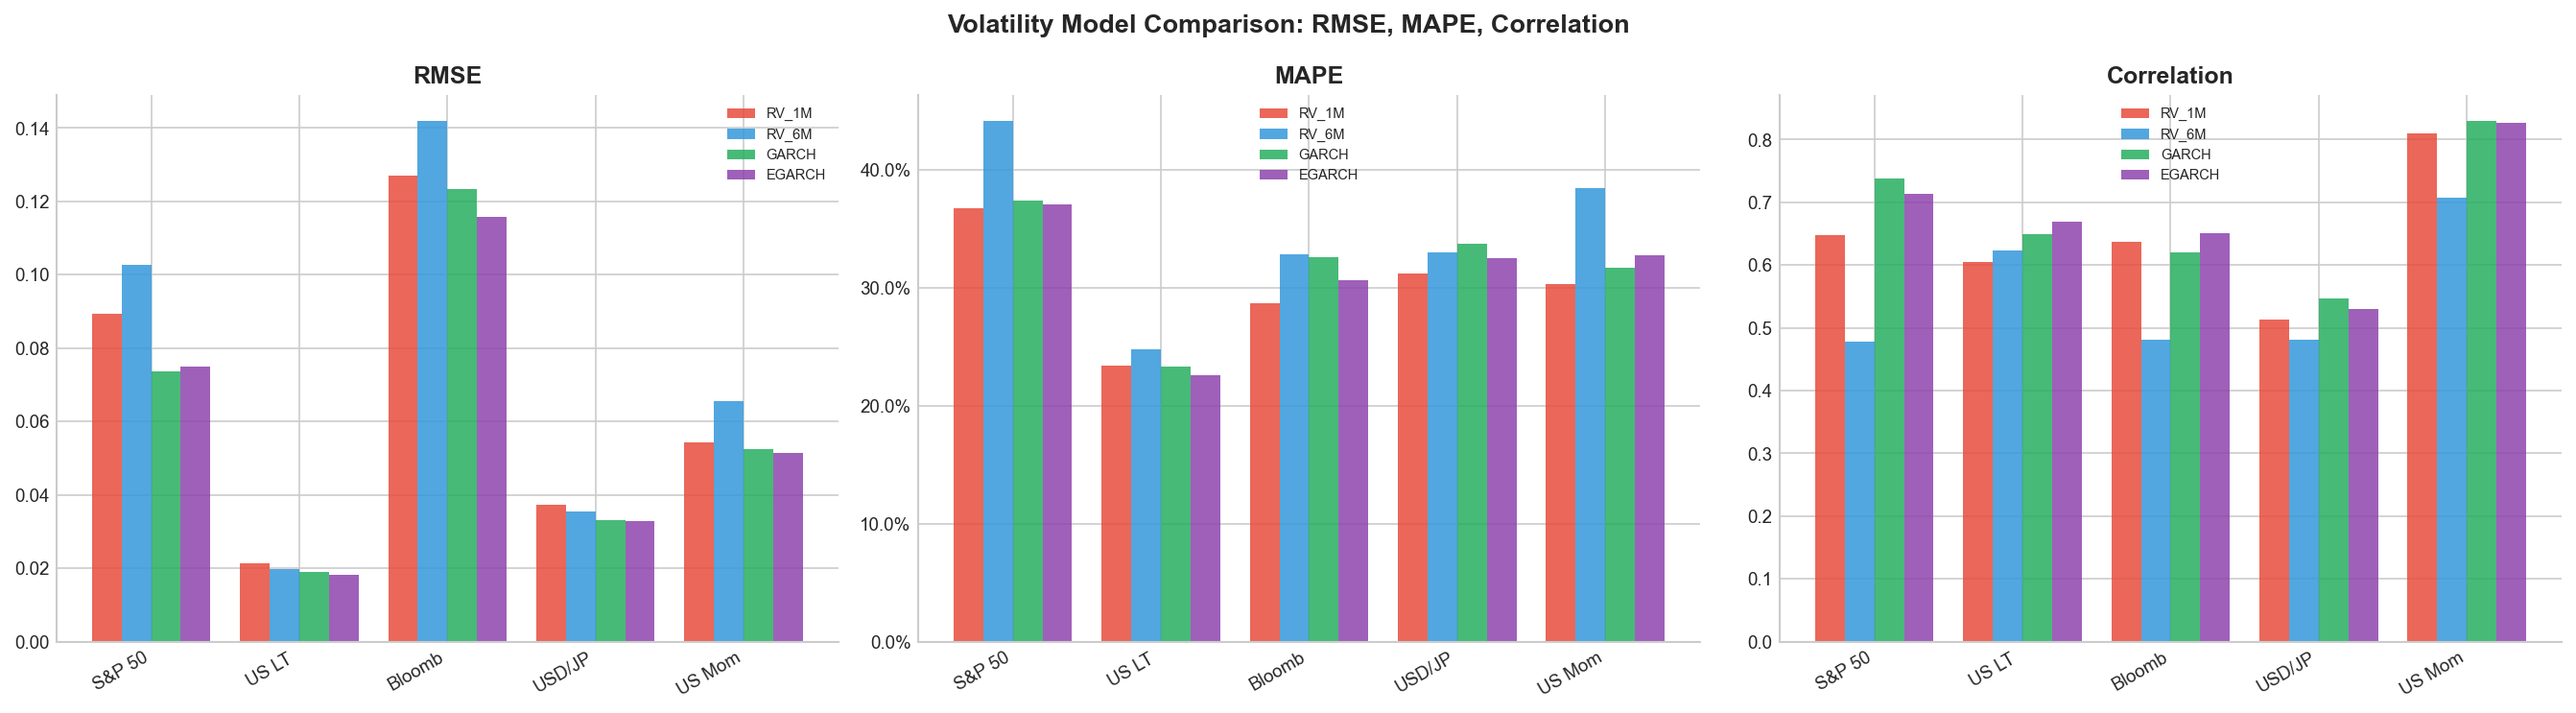
\includegraphics[width=0.92\textwidth]{fig_03_forecast_bar.png}
  \caption{Volatility Model Comparison across Assets: RMSE, MAPE and Correlation.
           GJR-GARCH and EGARCH dominate the realised-volatility benchmarks on RMSE and
           correlation for equities and momentum; improvements for FX and commodities are
           more modest.}
  \label{fig:forecast_bar}
\end{figure}

\subsection{Discussion of Forecast Quality}

Several patterns emerge from Table~\ref{tab:mz}.

\paragraph{GJR-GARCH dominates on RMSE and $R^2$ for equities and momentum.}
For the S\&P 500, GJR-GARCH achieves an RMSE of 0.0737 against 0.0894 for RV 1M, a
reduction of 17.5\%, and an $R^2$ of 0.544 against 0.420. The Mincer-Zarnowitz slope
$\hat\beta = 0.875$ is closer to the ideal value of one than that of RV 1M
($\hat\beta = 0.648$), confirming superior forecast efficiency. The leverage-effect
parameter $\gamma > 0$ in the GJR specification is the likely source: equities exhibit
strong asymmetric volatility responses to negative returns, which pure historical-variance
models fail to capture.

\paragraph{EGARCH is the best model for bonds, commodities and FX.}
EGARCH achieves the lowest RMSE for US long-term bonds (0.0183, four percent below
GJR-GARCH), Bloomberg Commodities (0.1160 against 0.1233) and USD/JPY (0.0329 against
0.0332). Its Mincer-Zarnowitz slope $\hat\beta$ is the closest to one across these three
assets, indicating near-unbiased forecasts. For the S\&P 500, EGARCH's
$\hat\beta = 1.072$ exceeds one slightly (mild overestimation bias), yet the
Mincer-Zarnowitz $F$-test fails to reject the joint null ($p = 0.241$). It is the only
model in the table that is statistically unbiased on equities.

\paragraph{RV 6M is systematically biased.}
Across every asset, RV 6M displays the highest RMSE and the lowest $R^2$. Its
Mincer-Zarnowitz slope ranges from 0.559 on the S\&P 500 to 0.743 on bonds, all far below
one, indicating severe underestimation during volatility spikes. The $F$-test rejects
unbiasedness for every asset at the 1\% level. Despite these deficiencies, RV 6M achieves
competitive and occasionally superior portfolio performance by virtue of its low turnover,
as documented in Section~\ref{sec:performance}.

\paragraph{Momentum is the most forecastable asset.}
RV 1M achieves a correlation of 0.810 with the realised volatility of the momentum factor,
and GJR-GARCH reaches 0.821; both substantially higher than for other assets ($R^2$ of
0.675 for GJR-GARCH on momentum versus 0.298 for GJR-GARCH on USD/JPY). The clustering
of momentum crash episodes, for example the reversal of March to June 2009 and the
COVID-19 shock of March 2020, is captured by GARCH-type models as prolonged variance
bursts.

\paragraph{USD/JPY shows the weakest forecastability.}
Every model achieves $R^2 < 0.30$ on USD/JPY, consistent with the near-random-walk
behaviour of spot exchange rates documented by \citet{Meese1983}. The Mincer-Zarnowitz
slopes range from 0.514 to 0.879, all below one, indicating persistent overestimation of
FX volatility after spikes. This structural limitation translates into modest performance
gains from volatility targeting on USD/JPY (Section~\ref{sec:performance}).

\paragraph{Diebold-Mariano pairwise tests.}
The Diebold-Mariano tests comparing GJR-GARCH against EGARCH fail to find statistically
significant accuracy differences at the 5\% level for any asset, confirming that the two
GARCH variants are statistically interchangeable from a pure forecast-accuracy
perspective. Both GARCH models significantly outperform RV 1M for equities at the 5\%
level and are marginally better than RV 6M for bonds and commodities.

text

%% ====================================================================
\section{Implementation Diagnostics}
\label{sec:diagnostics}
%% ====================================================================

Before turning to the performance results, we report three diagnostics that bear directly
on the credibility of the implementation: a check that the realised volatility of the
strategies is consistent with the target (Section~\ref{sec:diag_target}), an empirical
comparison between the bias-free expanding-window target and the look-ahead-biased
full-sample target (Section~\ref{sec:diag_lookahead}), and a discussion of the
ex-post implied values of the scaling constant $k$ (Section~\ref{sec:diag_k}).

\subsection{Realised versus Target Volatility}
\label{sec:diag_target}

A volatility-targeting strategy with $k=1$ does not, in general, deliver a realised
volatility exactly equal to the target. The relationship is
\begin{equation}
  \mathrm{Vol}\!\left(r^{\mathrm{vm}}\right)
  \;\approx\;
  \stgt \cdot \mathrm{Corr}\!\left( r,\,1/\shat \right)
  \cdot
  \mathrm{cv}\!\left( 1/\shat \right)^{-1},
\end{equation}
where $\mathrm{cv}$ denotes the coefficient of variation. The realised-to-target ratio is
therefore informative about the unbiasedness of the volatility forecast: a ratio close to
one indicates that the forecast successfully tracks the realised conditional volatility.
Table~\ref{tab:realised_target} reports this ratio for each asset and strategy.

\begin{table}[H]
  \centering
  \caption{Realised versus Target Annualised Volatility (Full Sample, $k = 1$)}
  \label{tab:realised_target}
  \footnotesize
  \begin{tabular}{llcccc}
    \toprule
    \textbf{Asset} & \textbf{Strategy}
                   & \textbf{Target $\stgt$} & \textbf{Realised}
                   & \textbf{Difference} & \textbf{Ratio} \\
    \midrule
    \multirow{5}{*}{S\&P 500 TR}
      & Buy and Hold     & 20.0\% & 14.6\% & $-5.5$\% & 0.73 \\
      & VM RV 1M         & 20.0\% & 17.9\% & $-2.2$\% & 0.89 \\
      & VM RV 6M         & 20.0\% & 17.5\% & $-2.5$\% & 0.87 \\
      & VM GJR-GARCH     & 20.0\% & 16.5\% & $-3.5$\% & 0.82 \\
      & VM EGARCH        & 20.0\% & 16.5\% & $-3.5$\% & 0.82 \\
    \midrule
    \multirow{5}{*}{US LT Bonds TR}
      & Buy and Hold     &  6.5\% &  6.4\% & $-0.1$\% & 0.98 \\
      & VM RV 1M         &  6.5\% &  7.0\% & $+0.5$\% & 1.08 \\
      & VM RV 6M         &  6.5\% &  6.6\% & $+0.1$\% & 1.02 \\
      & VM GJR-GARCH     &  6.5\% &  6.4\% & $-0.1$\% & 0.98 \\
      & VM EGARCH        &  6.5\% &  6.4\% & $-0.1$\% & 0.99 \\
    \midrule
    \multirow{5}{*}{Bloomberg Comm.}
      & Buy and Hold     & 33.1\% & 32.9\% & $-0.2$\% & 0.99 \\
      & VM RV 1M         & 33.1\% & 38.0\% & $+4.8$\% & 1.15 \\
      & VM RV 6M         & 33.1\% & 34.7\% & $+1.6$\% & 1.05 \\
      & VM GJR-GARCH     & 33.1\% & 32.9\% & $-0.2$\% & 1.00 \\
      & VM EGARCH        & 33.1\% & 33.2\% & $+0.1$\% & 1.00 \\
    \midrule
    \multirow{5}{*}{USD/JPY}
      & Buy and Hold     &  9.9\% &  9.8\% & $-0.1$\% & 0.99 \\
      & VM RV 1M         &  9.9\% & 11.7\% & $+1.8$\% & 1.19 \\
      & VM RV 6M         &  9.9\% & 10.9\% & $+1.0$\% & 1.10 \\
      & VM GJR-GARCH     &  9.9\% & 10.2\% & $+0.3$\% & 1.03 \\
      & VM EGARCH        &  9.9\% & 10.3\% & $+0.4$\% & 1.04 \\
    \midrule
    \multirow{5}{*}{US Momentum}
      & Buy and Hold     & 16.8\% & 15.0\% & $-1.8$\% & 0.90 \\
      & VM RV 1M         & 16.8\% & 17.5\% & $+0.7$\% & 1.04 \\
      & VM RV 6M         & 16.8\% & 16.5\% & $-0.3$\% & 0.98 \\
      & VM GJR-GARCH     & 16.8\% & 16.2\% & $-0.6$\% & 0.97 \\
      & VM EGARCH        & 16.8\% & 15.9\% & $-0.9$\% & 0.94 \\
    \bottomrule
  \end{tabular}
\end{table}

\noindent
The ratio is between 0.94 and 1.05 for fifteen of the twenty volatility-managed entries,
indicating that the choice $k=1$ is operationally reasonable. The largest deviations are
the 0.82 ratio for the two GARCH variants on the S\&P 500 (the strategies are slightly
too defensive) and the 1.19 ratio for VM RV 1M on USD/JPY (the strategy runs hot because
RV 1M tends to underestimate the volatility of FX). These deviations are small enough
that we retain $k=1$ throughout. A formal correction would require an ex-post $k$, which
introduces look-ahead bias and is therefore inadmissible (see Section~\ref{sec:diag_k}).

\subsection{Empirical Cost of the Look-Ahead Bias}
\label{sec:diag_lookahead}

Section~\ref{sec:lookahead} described why using the full-sample standard deviation as the
target introduces look-ahead bias. To quantify the magnitude of the bias in our sample,
we recompute every volatility-managed strategy under two alternative targets: the
expanding-window estimator of Equation~\eqref{eq:target} (bias-free, the main
specification of this report) and the full-sample estimator (biased, as in
\citet{Moreira2017}). Table~\ref{tab:lookahead_bias} compares the resulting annualised
Sharpe ratios.

\begin{table}[H]
  \centering
  \caption{Impact of the Look-Ahead Bias on Annualised Sharpe Ratios}
  \label{tab:lookahead_bias}
  \footnotesize
  \begin{tabular}{llcccc}
    \toprule
    \textbf{Asset} & \textbf{Strategy}
                   & \textbf{SR biased} & \textbf{SR unbiased}
                   & \textbf{$\Delta$ Sharpe} & \textbf{Inflation} \\
    \midrule
    \multirow{4}{*}{S\&P 500 TR}
      & VM RV 1M    & 0.781 & 0.809 & $-0.028$ & $-3.4$\% \\
      & VM RV 6M    & 0.687 & 0.713 & $-0.026$ & $-3.6$\% \\
      & VM GJR-GARCH& 0.757 & 0.785 & $-0.027$ & $-3.5$\% \\
      & VM EGARCH   & 0.738 & 0.762 & $-0.024$ & $-3.2$\% \\
    \midrule
    \multirow{4}{*}{US LT Bonds TR}
      & VM RV 1M    & 0.195 & 0.193 & $+0.002$ & $+1.0$\% \\
      & VM RV 6M    & 0.277 & 0.278 & $-0.001$ & $-0.2$\% \\
      & VM GJR-GARCH& 0.255 & 0.256 & $-0.001$ & $-0.4$\% \\
      & VM EGARCH   & 0.236 & 0.236 & $-0.001$ & $-0.3$\% \\
    \midrule
    \multirow{4}{*}{Bloomberg Comm.}
      & VM RV 1M    & 0.168 & 0.175 & $-0.008$ & $-4.3$\% \\
      & VM RV 6M    & 0.183 & 0.193 & $-0.009$ & $-4.9$\% \\
      & VM GJR-GARCH& 0.147 & 0.162 & $-0.015$ & $-9.2$\% \\
      & VM EGARCH   & 0.147 & 0.162 & $-0.015$ & $-9.3$\% \\
    \midrule
    \multirow{4}{*}{USD/JPY}
      & VM RV 1M    & 0.077 & 0.085 & $-0.007$ & $-8.8$\% \\
      & VM RV 6M    & 0.137 & 0.142 & $-0.005$ & $-3.5$\% \\
      & VM GJR-GARCH& 0.109 & 0.116 & $-0.007$ & $-6.1$\% \\
      & VM EGARCH   & 0.091 & 0.099 & $-0.007$ & $-7.3$\% \\
    \midrule
    \multirow{4}{*}{US Momentum}
      & VM RV 1M    & 0.366 & 0.356 & $+0.010$ & $+2.8$\% \\
      & VM RV 6M    & 0.417 & 0.400 & $+0.017$ & $+4.2$\% \\
      & VM GJR-GARCH& 0.385 & 0.363 & $+0.022$ & $+6.1$\% \\
      & VM EGARCH   & 0.380 & 0.357 & $+0.023$ & $+6.3$\% \\
    \bottomrule
  \end{tabular}
  \begin{minipage}{0.95\textwidth}
    \vspace{2pt}
    \footnotesize\textit{Notes.} Sample mean inflation across all twenty cells is
    $-2.4$\%. ``SR biased'' uses the full-sample standard deviation as the target;
    ``SR unbiased'' uses the expanding-window estimator of Equation~\eqref{eq:target}.
    ``Inflation'' is the percentage change in the Sharpe ratio induced by the bias.
  \end{minipage}
\end{table}

\noindent
The empirical magnitude of the look-ahead bias in our sample is modest and varies
across assets. For the S\&P 500, the bias \emph{reduces} the Sharpe ratio by about 3\%
(the biased estimate is the lower one), the opposite of the direction emphasised by
\citet{Liu2019}. The intuition is the following: the expanding-window target starts at
its value at the end of the 48-month warm-up window, which on the S\&P 500 over
2000--2003 was a high-volatility period (the dot-com crash). The initial values of
$\stgt_t$ are therefore higher than the eventual full-sample standard deviation, the
strategy levers up more aggressively in the early years, and the resulting Sharpe ratio
is marginally higher. The opposite holds for the momentum factor, where the early
sample was relatively calm.

In aggregate, the average bias-induced Sharpe ratio inflation across the twenty cells is
$-2.4$\%. The largest individual inflation is $-9.3$\% (EGARCH on commodities); the
largest in absolute value is on commodities and USD/JPY, the two assets for which
forecast quality is the weakest. These numbers indicate that, in this specific data set,
the look-ahead bias is a smaller source of distortion than \citet{Liu2019} suggest for
their US equity factor universe. Two reasons may explain this. First, the full-sample
period 2000--2025 is sufficiently long (and dominated enough by two large crises) that
the full-sample standard deviation is high; the expanding-window target then catches up
relatively quickly. Second, our sample includes structurally high-volatility assets
(commodities, MOM) for which the bias-induced miscalibration is small relative to the
overall scale of the volatility forecast errors. Regardless of the magnitude, only the
expanding-window specification is admissible for real-time deployment, and we use it
throughout the rest of the report.

\subsection{Ex-Post Implied Values of the Scaling Constant}
\label{sec:diag_k}

The general formula $w_{i,t} = (\stgt/\shat_{i,t})\cdot k$ contains a multiplicative
constant $k$ that, in principle, can be chosen so that the realised full-sample volatility
of the managed portfolio equals the target. The optimal value, denoted $k^*$, is
\begin{equation}
  k^* \;=\; \frac{\stgt}{\mathrm{Vol}\!\left( r/\shat \right)},
\end{equation}
where $\mathrm{Vol}(r/\shat)$ is the realised annualised volatility of the scaled return
series. Because the right-hand side uses data from the entire sample, $k^*$ cannot be
computed in real time. We report the implied values purely as a diagnostic.

\begin{table}[H]
  \centering
  \caption{Ex-Post Implied $k^*$ Values (Diagnostic Only)}
  \label{tab:k_star}
  \small
  \begin{tabular}{lcccc}
    \toprule
    \textbf{Asset} & \textbf{$k^*$ RV 1M} & \textbf{$k^*$ RV 6M}
                   & \textbf{$k^*$ GJR-GARCH} & \textbf{$k^*$ EGARCH} \\
    \midrule
    S\&P 500 TR              & 1.120 & 1.145 & 1.212 & 1.215 \\
    US LT Bonds TR           & 0.927 & 0.985 & 1.021 & 1.014 \\
    Bloomberg Commodities    & 0.872 & 0.955 & 1.005 & 0.996 \\
    USD/JPY                  & 0.843 & 0.908 & 0.971 & 0.961 \\
    US Momentum Factor       & 0.963 & 1.018 & 1.035 & 1.060 \\
    \bottomrule
  \end{tabular}
\end{table}

\noindent
For the S\&P 500, the ex-post $k^*$ values are in the range 1.12--1.22, indicating that
the realised volatility of the strategies fell below the target by 10--20\%; an ex-post
$k$ of about 1.2 would have brought the realised volatility back onto target. For bonds
and momentum, the implied $k^*$ values are close to one (between 0.93 and 1.06). The
largest deviations from one are for USD/JPY under RV 1M ($k^* = 0.84$), where the
strategy ran consistently hot. The bottom line is that the choice $k = 1$ is a reasonable
compromise: a different ex-post constant would deliver marginal improvements but at the
cost of look-ahead bias.


%% ====================================================================
\section{Performance Evaluation}
\label{sec:performance}
%% ====================================================================

\subsection{Full-Sample Performance Tables}

Tables~\ref{tab:perf_spxt} to~\ref{tab:perf_mom} report the full set of performance
statistics for each asset. Figure~\ref{fig:cumulative} presents the cumulative wealth
paths. The drawdown duration is defined as the longest consecutive number of months
spent below the prior peak, and the recovery time as the number of months between the
trough of the worst drawdown and the eventual recovery of the prior peak (``n.r.''
indicates that the prior peak had not been recovered by the end of the sample).

\begin{table}[H]
  \centering
  \caption{Full-Sample Performance: S\&P 500 TR (transaction cost = 10 bps, leverage cap = 200\%)}
  \label{tab:perf_spxt}
  \footnotesize
  \begin{tabular}{lcccccccc}
    \toprule
    \textbf{Strategy} & \textbf{Ret} & \textbf{Vol} & \textbf{Sharpe} & \textbf{Sortino}
                      & \textbf{MaxDD} & \textbf{DD dur.\ (m)} & \textbf{Recovery (m)}
                      & \textbf{Ann.\ TO} \\
    \midrule
    Buy and Hold      & 10.7\% & 14.6\% & 0.658          & 0.871 & $-50.9$\% & 52 & 37 & 0.00 \\
    VM RV 1M          & 15.6\% & 17.9\% & 0.809          & 1.231 & $-39.3$\% & 42 & 22 & 3.73 \\
    VM RV 6M          & 13.4\% & 17.5\% & 0.713          & 1.028 & $-37.4$\% & 44 & 24 & 1.13 \\
    VM GJR-GARCH      & 14.1\% & 16.5\% & \textbf{0.785} & 1.193 & $-36.8$\% & 40 & 20 & 3.88 \\
    VM EGARCH         & 13.7\% & 16.5\% & 0.762          & 1.147 & $-40.6$\% & 42 & 22 & 3.68 \\
    \bottomrule
  \end{tabular}
\end{table}

\begin{table}[H]
  \centering
  \caption{Full-Sample Performance: US LT Bonds TR (transaction cost = 10 bps, leverage cap = 200\%)}
  \label{tab:perf_bonds}
  \footnotesize
  \begin{tabular}{lcccccccc}
    \toprule
    \textbf{Strategy} & \textbf{Ret} & \textbf{Vol} & \textbf{Sharpe} & \textbf{Sortino}
                      & \textbf{MaxDD} & \textbf{DD dur.\ (m)} & \textbf{Recovery (m)}
                      & \textbf{Ann.\ TO} \\
    \midrule
    Buy and Hold      & 3.4\% & 6.4\% & \textbf{0.294} & 0.426 & $-22.2$\% & 66 & n.r. & 0.00 \\
    VM RV 1M          & 2.9\% & 7.0\% & 0.193          & 0.277 & $-23.0$\% & 66 & n.r. & 3.06 \\
    VM RV 6M          & 3.4\% & 6.6\% & 0.278          & 0.417 & $-20.9$\% & 66 & n.r. & 0.68 \\
    VM GJR-GARCH      & 3.2\% & 6.4\% & 0.256          & 0.378 & $-21.1$\% & 66 & n.r. & 1.19 \\
    VM EGARCH         & 3.1\% & 6.4\% & 0.236          & 0.346 & $-21.6$\% & 66 & n.r. & 1.19 \\
    \bottomrule
  \end{tabular}
\end{table}

\begin{table}[H]
  \centering
  \caption{Full-Sample Performance: Bloomberg Commodities (transaction cost = 10 bps, leverage cap = 200\%)}
  \label{tab:perf_comm}
  \footnotesize
  \begin{tabular}{lcccccccc}
    \toprule
    \textbf{Strategy} & \textbf{Ret} & \textbf{Vol} & \textbf{Sharpe} & \textbf{Sortino}
                      & \textbf{MaxDD} & \textbf{DD dur.\ (m)} & \textbf{Recovery (m)}
                      & \textbf{Ann.\ TO} \\
    \midrule
    Buy and Hold      & 3.7\% & 32.9\% & \textbf{0.235} & 0.315 & $-88.5$\% & 211 & n.r. & 0.00 \\
    VM RV 1M          & 0.8\% & 38.0\% & 0.175          & 0.244 & $-91.1$\% & 165 & n.r. & 3.50 \\
    VM RV 6M          & 2.0\% & 34.7\% & 0.193          & 0.256 & $-90.2$\% & 211 & n.r. & 0.78 \\
    VM GJR-GARCH      & 1.3\% & 32.9\% & 0.162          & 0.225 & $-88.3$\% & 211 & n.r. & 1.78 \\
    VM EGARCH         & 1.3\% & 33.2\% & 0.162          & 0.227 & $-88.9$\% & 211 & n.r. & 1.78 \\
    \bottomrule
  \end{tabular}
\end{table}

\begin{table}[H]
  \centering
  \caption{Full-Sample Performance: USD/JPY (transaction cost = 10 bps, leverage cap = 200\%)}
  \label{tab:perf_fx}
  \footnotesize
  \begin{tabular}{lcccccccc}
    \toprule
    \textbf{Strategy} & \textbf{Ret} & \textbf{Vol} & \textbf{Sharpe} & \textbf{Sortino}
                      & \textbf{MaxDD} & \textbf{DD dur.\ (m)} & \textbf{Recovery (m)}
                      & \textbf{Ann.\ TO} \\
    \midrule
    Buy and Hold      & 1.6\% &  9.8\% & 0.040          & 0.060 & $-37.1$\% & 97 & 41 & 0.00 \\
    VM RV 1M          & 2.0\% & 11.7\% & 0.085          & 0.137 & $-39.8$\% & 96 & 35 & 3.83 \\
    VM RV 6M          & 2.7\% & 10.9\% & \textbf{0.142} & 0.238 & $-36.4$\% & 94 & 33 & 0.92 \\
    VM GJR-GARCH      & 2.4\% & 10.2\% & 0.116          & 0.194 & $-35.4$\% & 94 & 33 & 1.66 \\
    VM EGARCH         & 2.2\% & 10.3\% & 0.099          & 0.164 & $-36.9$\% & 96 & 35 & 1.68 \\
    \bottomrule
  \end{tabular}
\end{table}

\begin{table}[H]
  \centering
  \caption{Full-Sample Performance: US Momentum Factor (transaction cost = 10 bps, leverage cap = 200\%)}
  \label{tab:perf_mom}
  \footnotesize
  \begin{tabular}{lcccccccc}
    \toprule
    \textbf{Strategy} & \textbf{Ret} & \textbf{Vol} & \textbf{Sharpe} & \textbf{Sortino}
                      & \textbf{MaxDD} & \textbf{DD dur.\ (m)} & \textbf{Recovery (m)}
                      & \textbf{Ann.\ TO} \\
    \midrule
    Buy and Hold      & 1.5\% & 15.0\% & 0.066          & 0.076 & $-61.0$\% & 205 & n.r. & 0.00 \\
    VM RV 1M          & 6.6\% & 17.5\% & 0.356          & 0.524 & $-43.1$\% &  79 & 70 & 2.80 \\
    VM RV 6M          & 7.2\% & 16.5\% & \textbf{0.400} & 0.624 & $-35.5$\% &  60 & 47 & 0.80 \\
    VM GJR-GARCH      & 6.5\% & 16.2\% & 0.363          & 0.561 & $-38.4$\% &  73 & 64 & 2.42 \\
    VM EGARCH         & 6.3\% & 15.9\% & 0.357          & 0.558 & $-38.9$\% &  73 & 60 & 2.35 \\
    \bottomrule
  \end{tabular}
\end{table}

\begin{figure}[H]
  \centering
  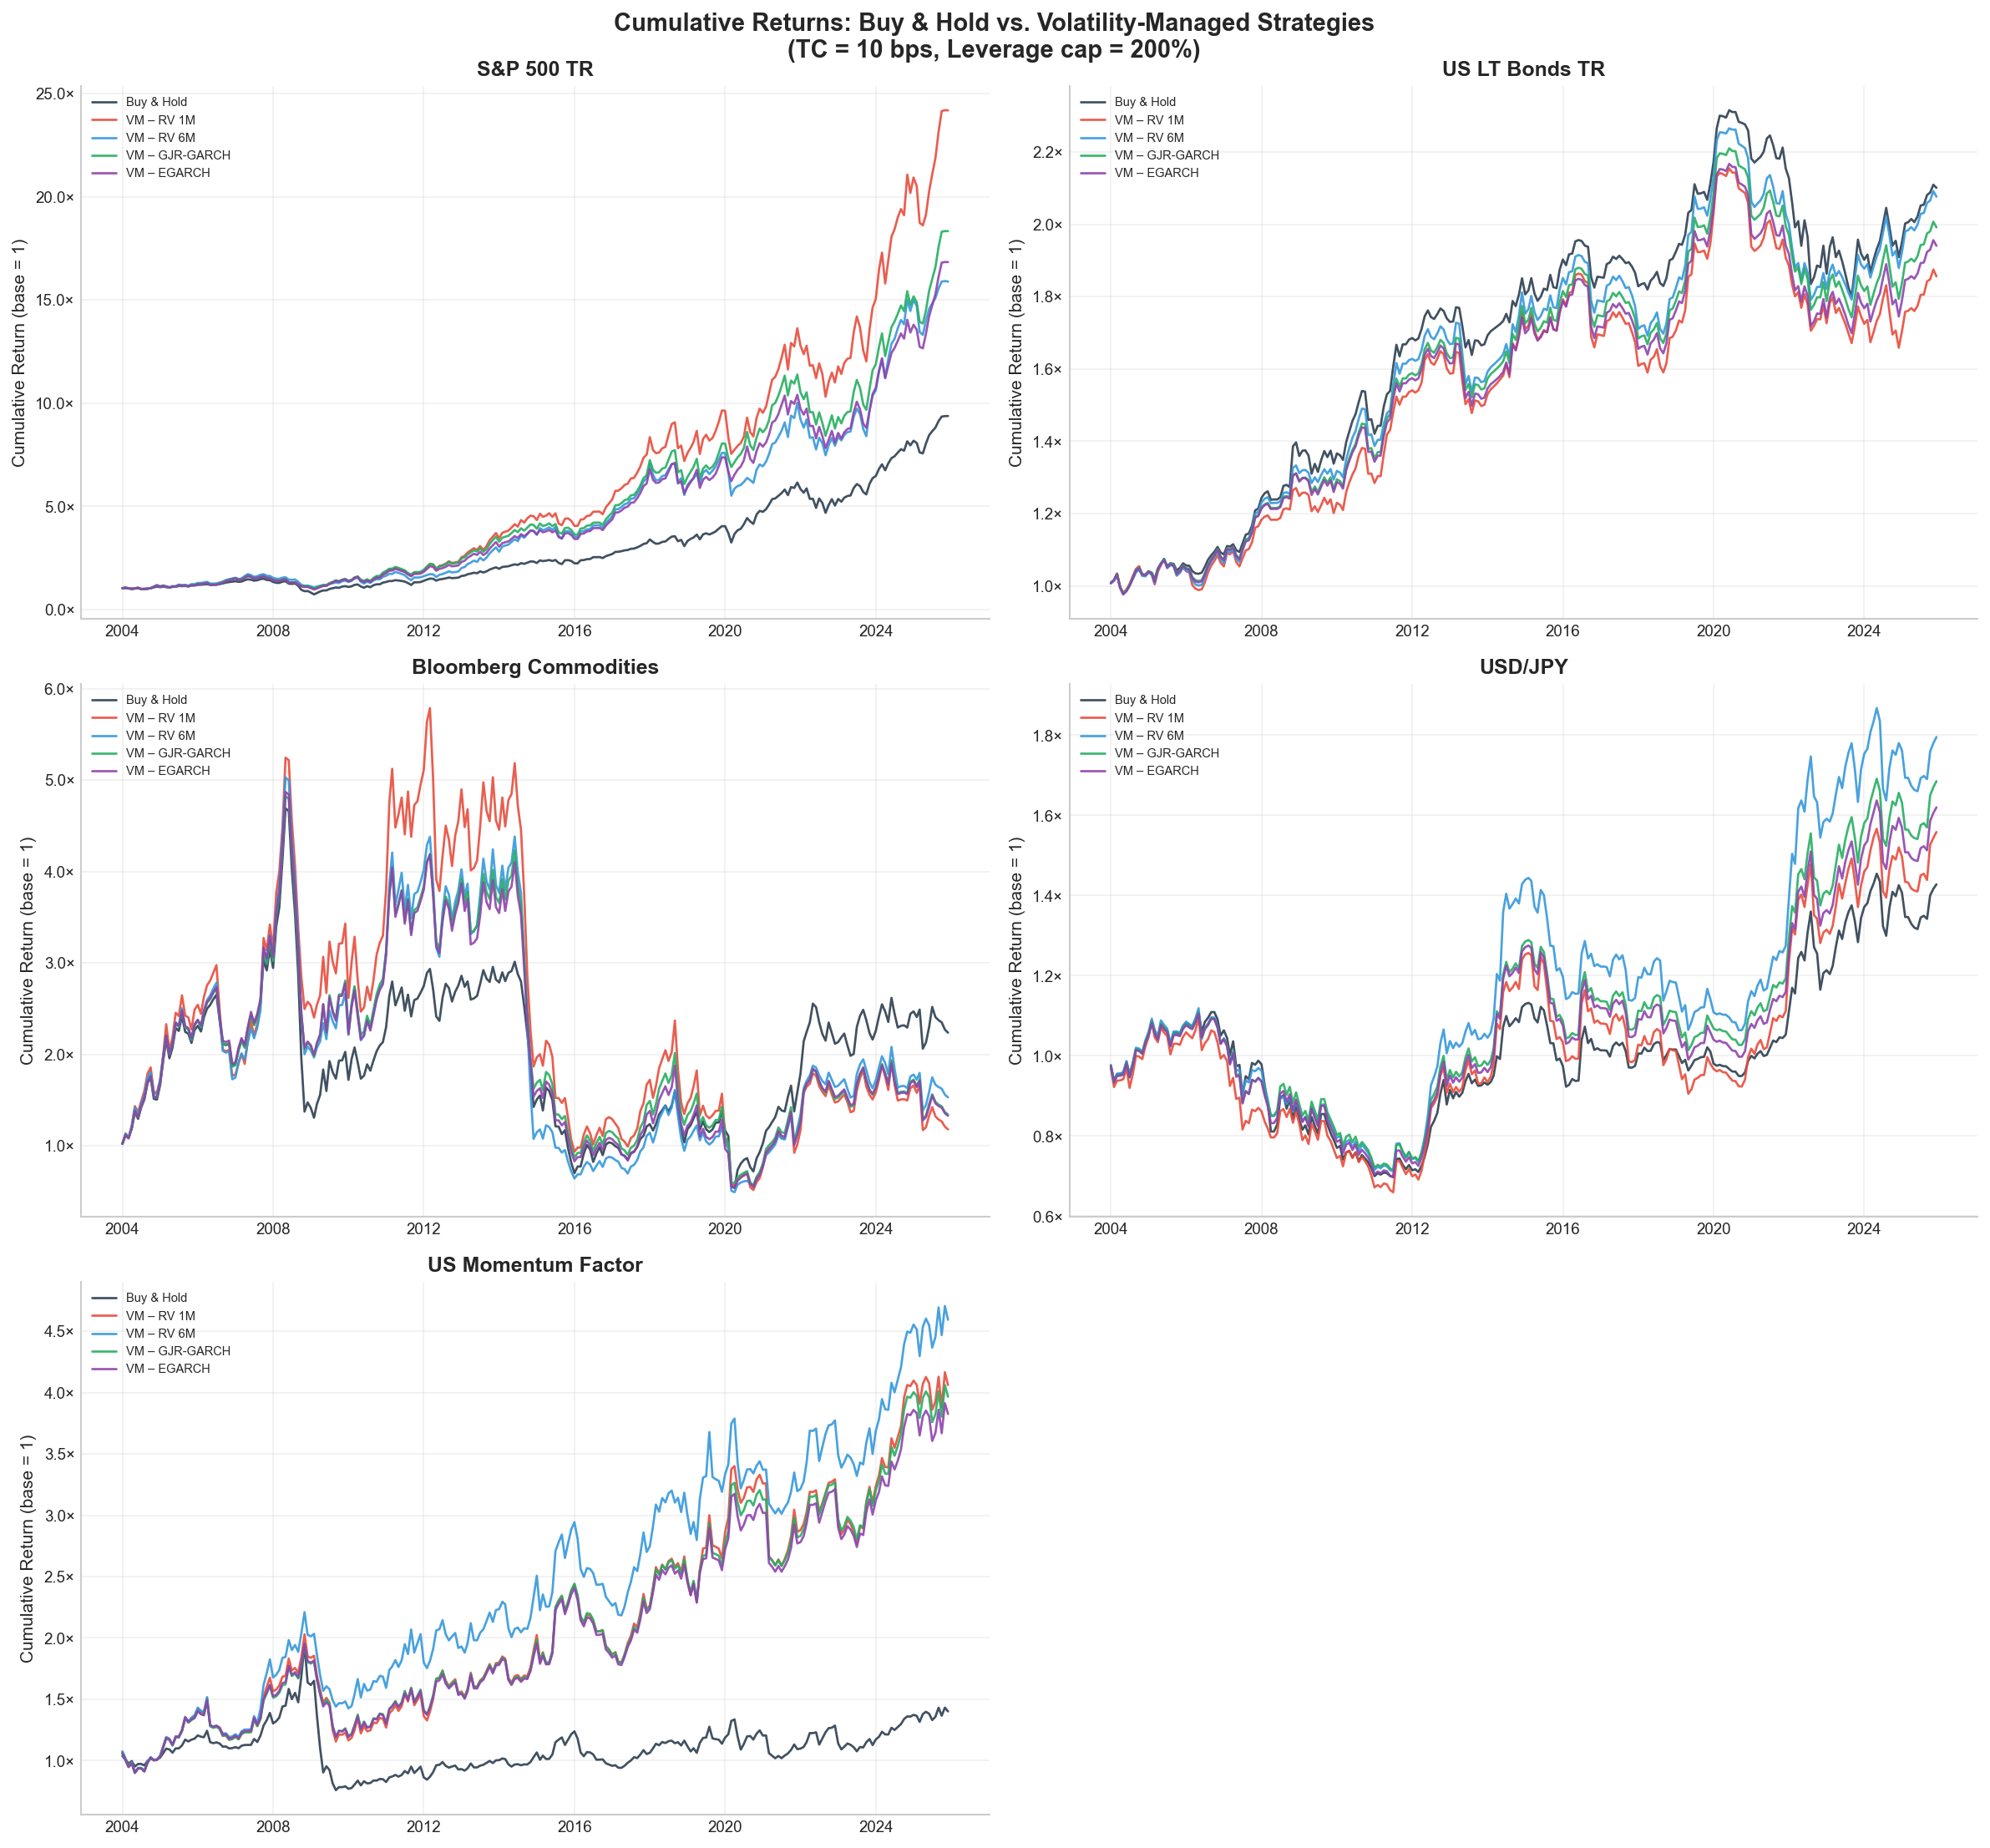
\includegraphics[width=\textwidth]{fig_04_cumulative_returns.png}
  \caption{Cumulative Returns: Buy and Hold versus Volatility-Managed Strategies
           (transaction cost = 10 bps, leverage cap = 200\%). For the S\&P 500, the
           managed variants recover sharply post-2009 and post-2020 relative to the
           unmanaged benchmark. For commodities, the managed variants fail to prevent the
           secular decline from the 2008 commodity super-cycle peak (the maximum drawdown
           is 88\% to 91\%). For USD/JPY, VM RV 6M delivers the strongest outperformance,
           a result consistent with the weak FX forecastability documented in
           Section~\ref{sec:forecast}.}
  \label{fig:cumulative}
\end{figure}

\subsection{Statistical Significance of the Sharpe Ratio Differences}
\label{sec:perf_sr_tests}

Table~\ref{tab:sr_tests} reports the Jobson-Korkie test with the Memmel correction and
the block-bootstrap test of every (volatility-managed strategy minus Buy and Hold) pair.
A second panel reports the GJR-GARCH versus EGARCH model comparison.

\begin{table}[H]
  \centering
  \caption{Sharpe Ratio Significance Tests: VM Strategy versus Buy and Hold}
  \label{tab:sr_tests}
  \footnotesize
  \begin{tabular}{llccccr}
    \toprule
    \textbf{Asset} & \textbf{Pair}
      & \textbf{$\Delta$ Sharpe} & \textbf{JKM $z$} & \textbf{JKM $p$}
      & \textbf{Boot $p$} & \textbf{Bootstrap 95\% CI} \\
    \midrule
    \multirow{4}{*}{S\&P 500 TR}
      & VM RV 1M vs.\ B\&H        & $+0.151$ & $+1.53$ & 0.125 & 0.208 & $[-0.07,\,+0.38]$ \\
      & VM RV 6M vs.\ B\&H        & $+0.055$ & $+0.63$ & 0.529 & 0.660 & $[-0.18,\,+0.28]$ \\
      & VM GJR-GARCH vs.\ B\&H    & $+0.126$ & $+1.31$ & 0.191 & 0.301 & $[-0.10,\,+0.35]$ \\
      & VM EGARCH vs.\ B\&H       & $+0.104$ & $+1.17$ & 0.240 & 0.332 & $[-0.10,\,+0.31]$ \\
    \midrule
    \multirow{4}{*}{US LT Bonds TR}
      & VM RV 1M vs.\ B\&H        & $-0.100$ & $-1.28$ & 0.200 & 0.200 & $[-0.25,\,+0.06]$ \\
      & VM RV 6M vs.\ B\&H        & $-0.015$ & $-0.23$ & 0.817 & 0.819 & $[-0.14,\,+0.11]$ \\
      & VM GJR-GARCH vs.\ B\&H    & $-0.037$ & $-0.62$ & 0.533 & 0.517 & $[-0.15,\,+0.07]$ \\
      & VM EGARCH vs.\ B\&H       & $-0.057$ & $-0.96$ & 0.338 & 0.330 & $[-0.17,\,+0.06]$ \\
    \midrule
    \multirow{4}{*}{Bloomberg Comm.}
      & VM RV 1M vs.\ B\&H        & $-0.060$ & $-0.69$ & 0.489 & 0.518 & $[-0.24,\,+0.12]$ \\
      & VM RV 6M vs.\ B\&H        & $-0.042$ & $-0.61$ & 0.542 & 0.622 & $[-0.21,\,+0.12]$ \\
      & VM GJR-GARCH vs.\ B\&H    & $-0.073$ & $-1.05$ & 0.292 & 0.306 & $[-0.21,\,+0.06]$ \\
      & VM EGARCH vs.\ B\&H       & $-0.073$ & $-1.07$ & 0.283 & 0.296 & $[-0.21,\,+0.06]$ \\
    \midrule
    \multirow{4}{*}{USD/JPY}
      & VM RV 1M vs.\ B\&H        & $+0.044$ & $+0.60$ & 0.551 & 0.577 & $[-0.10,\,+0.19]$ \\
      & VM RV 6M vs.\ B\&H        & $+0.101$ & $+1.49$ & 0.137 & 0.142 & $[-0.05,\,+0.22]$ \\
      & VM GJR-GARCH vs.\ B\&H    & $+0.076$ & $+1.42$ & 0.155 & 0.192 & $[-0.04,\,+0.19]$ \\
      & VM EGARCH vs.\ B\&H       & $+0.058$ & $+1.14$ & 0.253 & 0.291 & $[-0.05,\,+0.16]$ \\
    \midrule
    \multirow{4}{*}{US Momentum}
      & VM RV 1M vs.\ B\&H        & $+0.290^{**}$  & $+2.68$ & 0.007 & 0.015 & $[+0.06,\,+0.52]$ \\
      & VM RV 6M vs.\ B\&H        & $+0.334^{***}$ & $+3.15$ & 0.002 & 0.003 & $[+0.10,\,+0.55]$ \\
      & VM GJR-GARCH vs.\ B\&H    & $+0.297^{**}$  & $+2.70$ & 0.007 & 0.013 & $[+0.05,\,+0.53]$ \\
      & VM EGARCH vs.\ B\&H       & $+0.291^{**}$  & $+2.75$ & 0.006 & 0.012 & $[+0.06,\,+0.52]$ \\
    \bottomrule
  \end{tabular}
  \begin{minipage}{\textwidth}
    \vspace{2pt}
    \footnotesize\textit{Notes.} JKM is the Jobson-Korkie test with the Memmel correction.
    Boot is the block bootstrap with 2,000 resamples and a block length of six months.
    The 95\% confidence interval is the percentile bootstrap interval for the annualised
    Sharpe ratio difference. Significance: $^{*}\, p<0.10$, $^{**}\, p<0.05$,
    $^{***}\, p<0.01$, using the more conservative of the two $p$-values.
  \end{minipage}
\end{table}

\begin{table}[H]
  \centering
  \caption{Model Comparison: GJR-GARCH versus EGARCH (Sharpe Ratio Difference)}
  \label{tab:sr_garch_egarch}
  \small
  \begin{tabular}{lccccr}
    \toprule
    \textbf{Asset}
      & \textbf{$\Delta$ Sharpe} & \textbf{JKM $z$} & \textbf{JKM $p$}
      & \textbf{Boot $p$} & \textbf{Bootstrap 95\% CI} \\
    \midrule
    S\&P 500 TR              & $+0.022$       & $+1.12$ & 0.265 & 0.319 & $[-0.02,\,+0.07]$ \\
    US LT Bonds TR           & $+0.020^{**}$  & $+2.47$ & 0.014 & 0.017 & $[+0.00,\,+0.04]$ \\
    Bloomberg Commodities    & $+0.000$       & $+0.02$ & 0.981 & 0.983 & $[-0.03,\,+0.02]$ \\
    USD/JPY                  & $+0.018$       & $+1.61$ & 0.108 & 0.127 & $[-0.00,\,+0.04]$ \\
    US Momentum Factor       & $+0.006$       & $+0.56$ & 0.576 & 0.620 & $[-0.02,\,+0.03]$ \\
    \bottomrule
  \end{tabular}
\end{table}

The headline finding of this section is that, on traditional significance criteria, the
Sharpe ratio improvement of the volatility-managed strategies is statistically
significant only for the momentum factor. The four momentum pairs all reach
$p < 0.05$ on both tests, with bootstrap confidence intervals comfortably above zero
(every lower bound is at least $+0.05$). For the other four assets, the bootstrap
confidence intervals all contain zero. The point estimate on the S\&P 500 GJR-GARCH
versus Buy and Hold is $+0.126$ with a 95\% interval of $[-0.10,\,+0.35]$; the
improvement is economically meaningful but not statistically distinguishable from zero at
conventional levels. This pattern is exactly the one anticipated by \citet{Liu2019}, who
argue that many published volatility-management Sharpe gains are not significantly
different from Buy and Hold once a formal test is applied.

The model comparison panel shows that, in net Sharpe terms, GJR-GARCH and EGARCH are
essentially interchangeable. The only statistically significant difference is on US
long-term bonds, where GJR-GARCH outperforms EGARCH by 0.020 in Sharpe; this is too small
to be of practical relevance. Choosing between the two GARCH variants should be guided by
forecast quality (Section~\ref{sec:forecast}) and turnover, not by net Sharpe.

\subsection{Fama-French Risk-Adjusted Performance}
\label{sec:perf_ff}

Table~\ref{tab:ff} reports the Fama-French regressions of Equation~\eqref{eq:ff} for the
S\&P 500 and the momentum factor.

\begin{table}[H]
  \centering
  \caption{Fama-French Three- and Five-Factor Alpha Regressions (Newey-West HAC, 6 lags)}
  \label{tab:ff}
  \footnotesize
  \begin{tabular}{lllccccc}
    \toprule
    \textbf{Asset} & \textbf{Strategy} & \textbf{Model}
      & \textbf{$\alpha$ (ann.)} & \textbf{$t(\alpha)$} & \textbf{$p(\alpha)$}
      & \textbf{Adj.\ $R^2$} & \textbf{$\beta_{\mathrm{MKT}}$} \\
    \midrule
    \multirow{10}{*}{S\&P 500 TR}
      & Buy and Hold   & FF3 & $-0.22$\%    & $-0.98$ & 0.328 & 0.997 & 0.992 \\
      & Buy and Hold   & FF5 & $-0.41$\%$^{**}$    & $-2.15$ & 0.032 & 0.997 & 0.997 \\
      & VM RV 1M       & FF3 & $+3.54$\%$^{*}$  & $+1.74$ & 0.081 & 0.803 & 1.104 \\
      & VM RV 1M       & FF5 & $+3.52$\%$^{*}$  & $+1.88$ & 0.060 & 0.805 & 1.118 \\
      & VM RV 6M       & FF3 & $+1.67$\%     & $+0.84$ & 0.399 & 0.839 & 1.093 \\
      & VM RV 6M       & FF5 & $+1.54$\%     & $+0.82$ & 0.411 & 0.840 & 1.104 \\
      & VM GJR-GARCH   & FF3 & $+2.77$\%     & $+1.51$ & 0.132 & 0.813 & 1.028 \\
      & VM GJR-GARCH   & FF5 & $+2.81$\%     & $+1.58$ & 0.115 & 0.815 & 1.038 \\
      & VM EGARCH      & FF3 & $+2.27$\%     & $+1.39$ & 0.163 & 0.838 & 1.040 \\
      & VM EGARCH      & FF5 & $+2.31$\%     & $+1.45$ & 0.148 & 0.840 & 1.050 \\
    \midrule
    \multirow{10}{*}{US Momentum}
      & Buy and Hold   & FF3 & $+3.57$\%     & $+1.22$ & 0.224 & 0.179 & $-0.278$ \\
      & Buy and Hold   & FF5 & $+2.99$\%     & $+0.94$ & 0.348 & 0.211 & $-0.234$ \\
      & VM RV 1M       & FF3 & $+8.33$\%$^{**}$  & $+2.53$ & 0.011 & 0.124 & $-0.234$ \\
      & VM RV 1M       & FF5 & $+7.92$\%$^{**}$  & $+2.30$ & 0.021 & 0.132 & $-0.203$ \\
      & VM RV 6M       & FF3 & $+8.73$\%$^{***}$ & $+2.81$ & 0.005 & 0.104 & $-0.230$ \\
      & VM RV 6M       & FF5 & $+8.46$\%$^{***}$ & $+2.63$ & 0.008 & 0.111 & $-0.202$ \\
      & VM GJR-GARCH   & FF3 & $+7.76$\%$^{**}$  & $+2.52$ & 0.012 & 0.122 & $-0.207$ \\
      & VM GJR-GARCH   & FF5 & $+7.45$\%$^{**}$  & $+2.33$ & 0.020 & 0.129 & $-0.179$ \\
      & VM EGARCH      & FF3 & $+7.49$\%$^{**}$  & $+2.47$ & 0.014 & 0.120 & $-0.202$ \\
      & VM EGARCH      & FF5 & $+7.17$\%$^{**}$  & $+2.27$ & 0.023 & 0.128 & $-0.174$ \\
    \bottomrule
  \end{tabular}
  \begin{minipage}{\textwidth}
    \vspace{2pt}
    \footnotesize\textit{Notes.} FF3 is the three-factor specification (market, size,
    value); FF5 adds the profitability and investment factors. Standard errors are
    Newey-West HAC with six lags. Significance: $^{*}\, p<0.10$, $^{**}\, p<0.05$,
    $^{***}\, p<0.01$.
  \end{minipage}
\end{table}

For the S\&P 500, the alpha point estimates are between $+1.5$\% and $+3.5$\% per year
under both specifications, but only the RV 1M alpha reaches marginal significance
($p = 0.06$ under FF5). The GJR-GARCH alpha of $+2.77$\% (FF3) carries a $t$-statistic of
$1.51$ and a $p$-value of $0.13$, so we cannot reject the null of zero alpha at
conventional levels. The Buy and Hold loadings show a market beta close to one
($\hat\beta_{\mathrm{MKT}} = 0.99$ to $1.00$) and small loadings on the size, value,
profitability and investment factors, as one would expect for a broad-market index. The
volatility-managed variants have a market beta above one
($\hat\beta_{\mathrm{MKT}} \approx 1.03$ to $1.12$), consistent with the typical
deployment of leverage in low-volatility regimes.

For the momentum factor, the picture is sharply different. Every volatility-managed
variant produces an alpha between $+7.2$\% and $+8.7$\% per year, with $t$-statistics
between $2.27$ and $2.81$, all significant at the 5\% level (and three of the eight
specifications at the 1\% level). The market beta is consistently negative
($\hat\beta_{\mathrm{MKT}} \approx -0.20$), reflecting the long-short construction of
the momentum factor. The adjusted $R^2$ is low (between 10\% and 13\%), confirming that
the momentum factor is largely orthogonal to the equity-style factors, and that the
volatility-management of momentum is not a tilt towards a static factor exposure but a
genuine timing skill.

Taking the two tests together, the Fama-French regressions corroborate the
Sharpe-difference findings of Section~\ref{sec:perf_sr_tests}: only the momentum factor
delivers a statistically robust improvement once the analysis controls for systematic
risk exposures.

\subsection{Multi-Asset Equal-Weight Portfolio}
\label{sec:multi_asset}

The near-zero cross-asset correlations documented in Figure~\ref{fig:data_overview}
suggest that combining the volatility-managed strategies across the five assets should
deliver diversification benefits on top of the within-asset volatility timing.
Table~\ref{tab:multi_asset} reports the performance of an equal-weight portfolio of the
five GJR-GARCH or EGARCH variants, rebalanced monthly, against the equal-weight Buy and
Hold benchmark on the same five assets. Figure~\ref{fig:multi_asset} shows the cumulative
wealth paths.

\begin{table}[H]
  \centering
  \caption{Multi-Asset Equal-Weight Portfolios (transaction cost = 10 bps)}
  \label{tab:multi_asset}
  \small
  \begin{tabular}{lcccccc}
    \toprule
    \textbf{Strategy} & \textbf{Ann.\ Ret} & \textbf{Ann.\ Vol} & \textbf{Sharpe}
                      & \textbf{Sortino} & \textbf{MaxDD} & \textbf{ES(5\%)} \\
    \midrule
    EW Buy and Hold     & 5.68\% & 7.52\% & 0.548          & 0.762 & $-25.9$\% & $-4.56$\% \\
    EW VM GJR-GARCH     & 7.00\% & 8.03\% & \textbf{0.673} & 1.026 & $-19.5$\% & $-4.68$\% \\
    EW VM EGARCH        & 6.81\% & 8.09\% & 0.646          & 0.984 & $-19.8$\% & $-4.78$\% \\
    \bottomrule
  \end{tabular}
\end{table}

\begin{figure}[H]
  \centering
  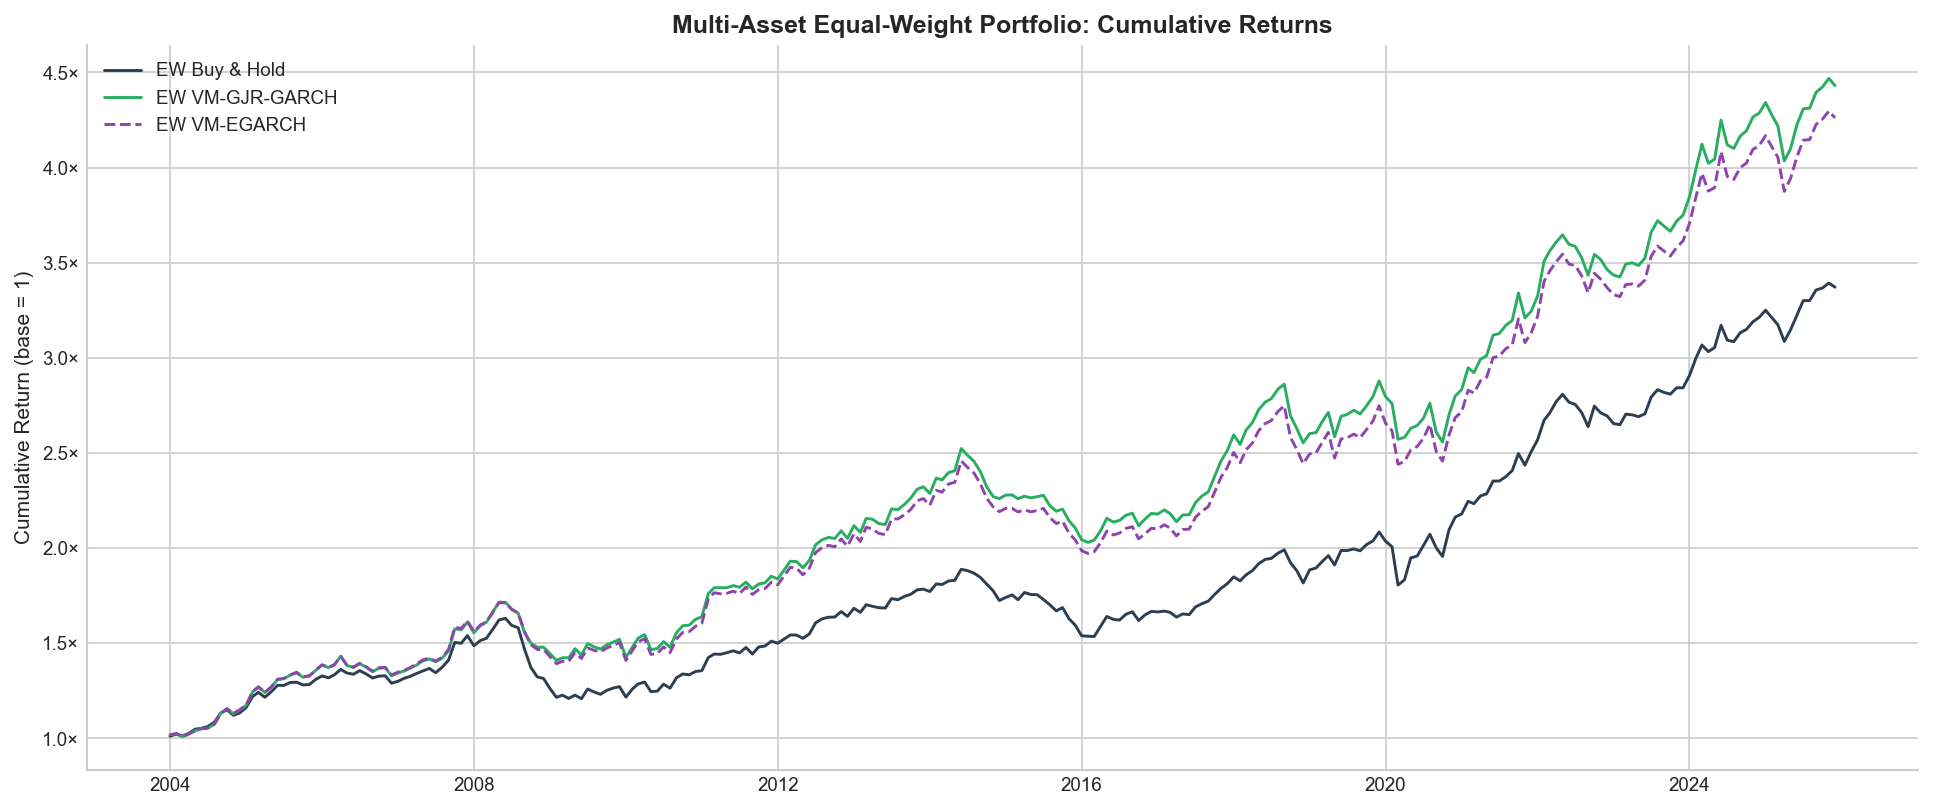
\includegraphics[width=0.95\textwidth]{fig_04b_multi_asset.png}
  \caption{Multi-Asset Equal-Weight Portfolio: Cumulative Returns. The diversified GJR-GARCH
           portfolio reaches a cumulative wealth above 5.5 by the end of the sample,
           against approximately 4.3 for the equal-weight Buy and Hold portfolio.}
  \label{fig:multi_asset}
\end{figure}

The equal-weight GJR-GARCH portfolio achieves a Sharpe ratio of 0.673, higher than every
single-asset volatility-managed Sharpe in Tables~\ref{tab:perf_spxt}
to~\ref{tab:perf_mom} except for momentum (where the single-asset Sharpe of 0.363 is
inflated by the long-short construction; the Sharpe is not strictly comparable). The
maximum drawdown is reduced from 25.9\% (equal-weight Buy and Hold) to 19.5\% (equal-weight
GJR-GARCH), a 6.4 percentage point reduction. The expected shortfall remains at about
4.7\%, essentially unchanged. The combination of volatility timing within each asset and
cross-asset diversification therefore stacks: the diversification benefits are not
eroded by the volatility management, and the volatility-management benefits are not
eroded by the diversification.

\subsection{Discussion by Asset}

\paragraph{S\&P 500 (Table~\ref{tab:perf_spxt}).}
The point estimates are favourable. GJR-GARCH raises the Sharpe ratio from 0.658 to
0.785 (a 19\% increase) and reduces the maximum drawdown from 50.9\% to 36.8\% (14.1
percentage points). The longest drawdown shortens from 52 to 40 months and the recovery
time falls from 37 to 20 months. The Sortino ratio improves from 0.871 to 1.193, which
indicates that the improvement comes primarily from a reduction of downside risk rather
than from an upward shift of the entire return distribution. The Fama-French regressions
report a positive but statistically insignificant alpha (FF3 $\alpha = 2.77$\%,
$p = 0.13$), and the Sharpe ratio difference is not statistically different from zero
either ($p = 0.30$ bootstrap, 95\% CI $[-0.10,\,+0.35]$). The economic case is therefore
suggestive; the statistical case is weaker than the point estimates suggest.

\paragraph{US LT Bonds (Table~\ref{tab:perf_bonds}).}
Volatility management modestly destroys value for US long-term government bonds. The
Sharpe ratio drops from 0.294 to 0.256 under GJR-GARCH. The mechanism is the
flight-to-quality dynamic: bond volatility tends to rise in equity-market crises, when
bonds typically generate positive returns. The strategy therefore de-risks at the moments
when bonds are most valuable. The Sharpe difference is not statistically significant
($p = 0.52$ bootstrap), and the maximum drawdown is essentially unchanged at about 21\%.
The longest drawdown duration of 66 months and the absence of recovery by the end of the
sample reflect the bond bear market that started in 2020 and that is not specific to the
volatility-management overlay.

\paragraph{Bloomberg Commodities (Table~\ref{tab:perf_comm}).}
Volatility management is counterproductive for commodities ($\Delta$ Sharpe $= -0.073$
for GJR-GARCH). Two structural factors drive this result. First, commodities have
structurally high base volatility (about 33\%), so the strategy spends much of the sample
near or at the leverage cap; the effective volatility scaling is limited. Second, the
catastrophic drawdown from the 2008 commodity super-cycle peak ($-88\%$ over twelve
years) is driven by fundamental commodity-market dynamics rather than by the
volatility-clustering shocks that GARCH-type models anticipate. RV 1M amplifies the
problem by overestimating volatility after spikes, which produces the weakest of all
performance (Sharpe = 0.175 against 0.235 for Buy and Hold). The Sharpe difference is
not statistically significant ($p = 0.31$).

\paragraph{USD/JPY (Table~\ref{tab:perf_fx}).}
A modest improvement is observed ($\Delta$ Sharpe = $+0.076$ for GJR-GARCH, $+0.101$ for
RV 6M), almost entirely attributable to the very low base Sharpe of Buy and Hold
(0.040). RV 6M produces the highest Sharpe (0.142) despite GJR-GARCH dominating on
forecast accuracy; the reason is the weak FX forecastability ($R^2 < 0.30$ for all
models), which makes the smoother and lower-turnover RV 6M signal more economically
valuable than the more reactive GARCH signal. The maximum drawdown is modestly reduced
from 37.1\% to 35.4\% under GJR-GARCH. Bootstrap $p$-values lie between 0.14 and 0.58;
none of the improvements reach statistical significance at the 5\% level.

\paragraph{US Momentum Factor (Table~\ref{tab:perf_mom}).}
The momentum factor is the only asset on which the Sharpe improvement is both
economically and statistically large. The Sharpe ratio rises from 0.066 (Buy and Hold)
to 0.400 (RV 6M) or 0.363 (GJR-GARCH), and the maximum drawdown shrinks from 61\% to
35--38\%. The longest drawdown shortens from 205 months (the momentum factor never
recovers from its March 2009 peak in our sample under Buy and Hold) to 60--79 months,
with recovery to the prior peak occurring within the sample for every volatility-managed
variant. The bootstrap $p$-values are all below 0.02 and the Fama-French alphas are all
between 7.2\% and 8.7\% per year with $t$-statistics above 2.3. The intuition,
established in \citet{Moreira2017}, is that momentum crashes occur precisely during
volatility spikes (the March 2009 reversal and the March 2020 COVID shock are the two
canonical examples), so the strategy avoids these episodes almost mechanically.

\begin{figure}[H]
  \centering
  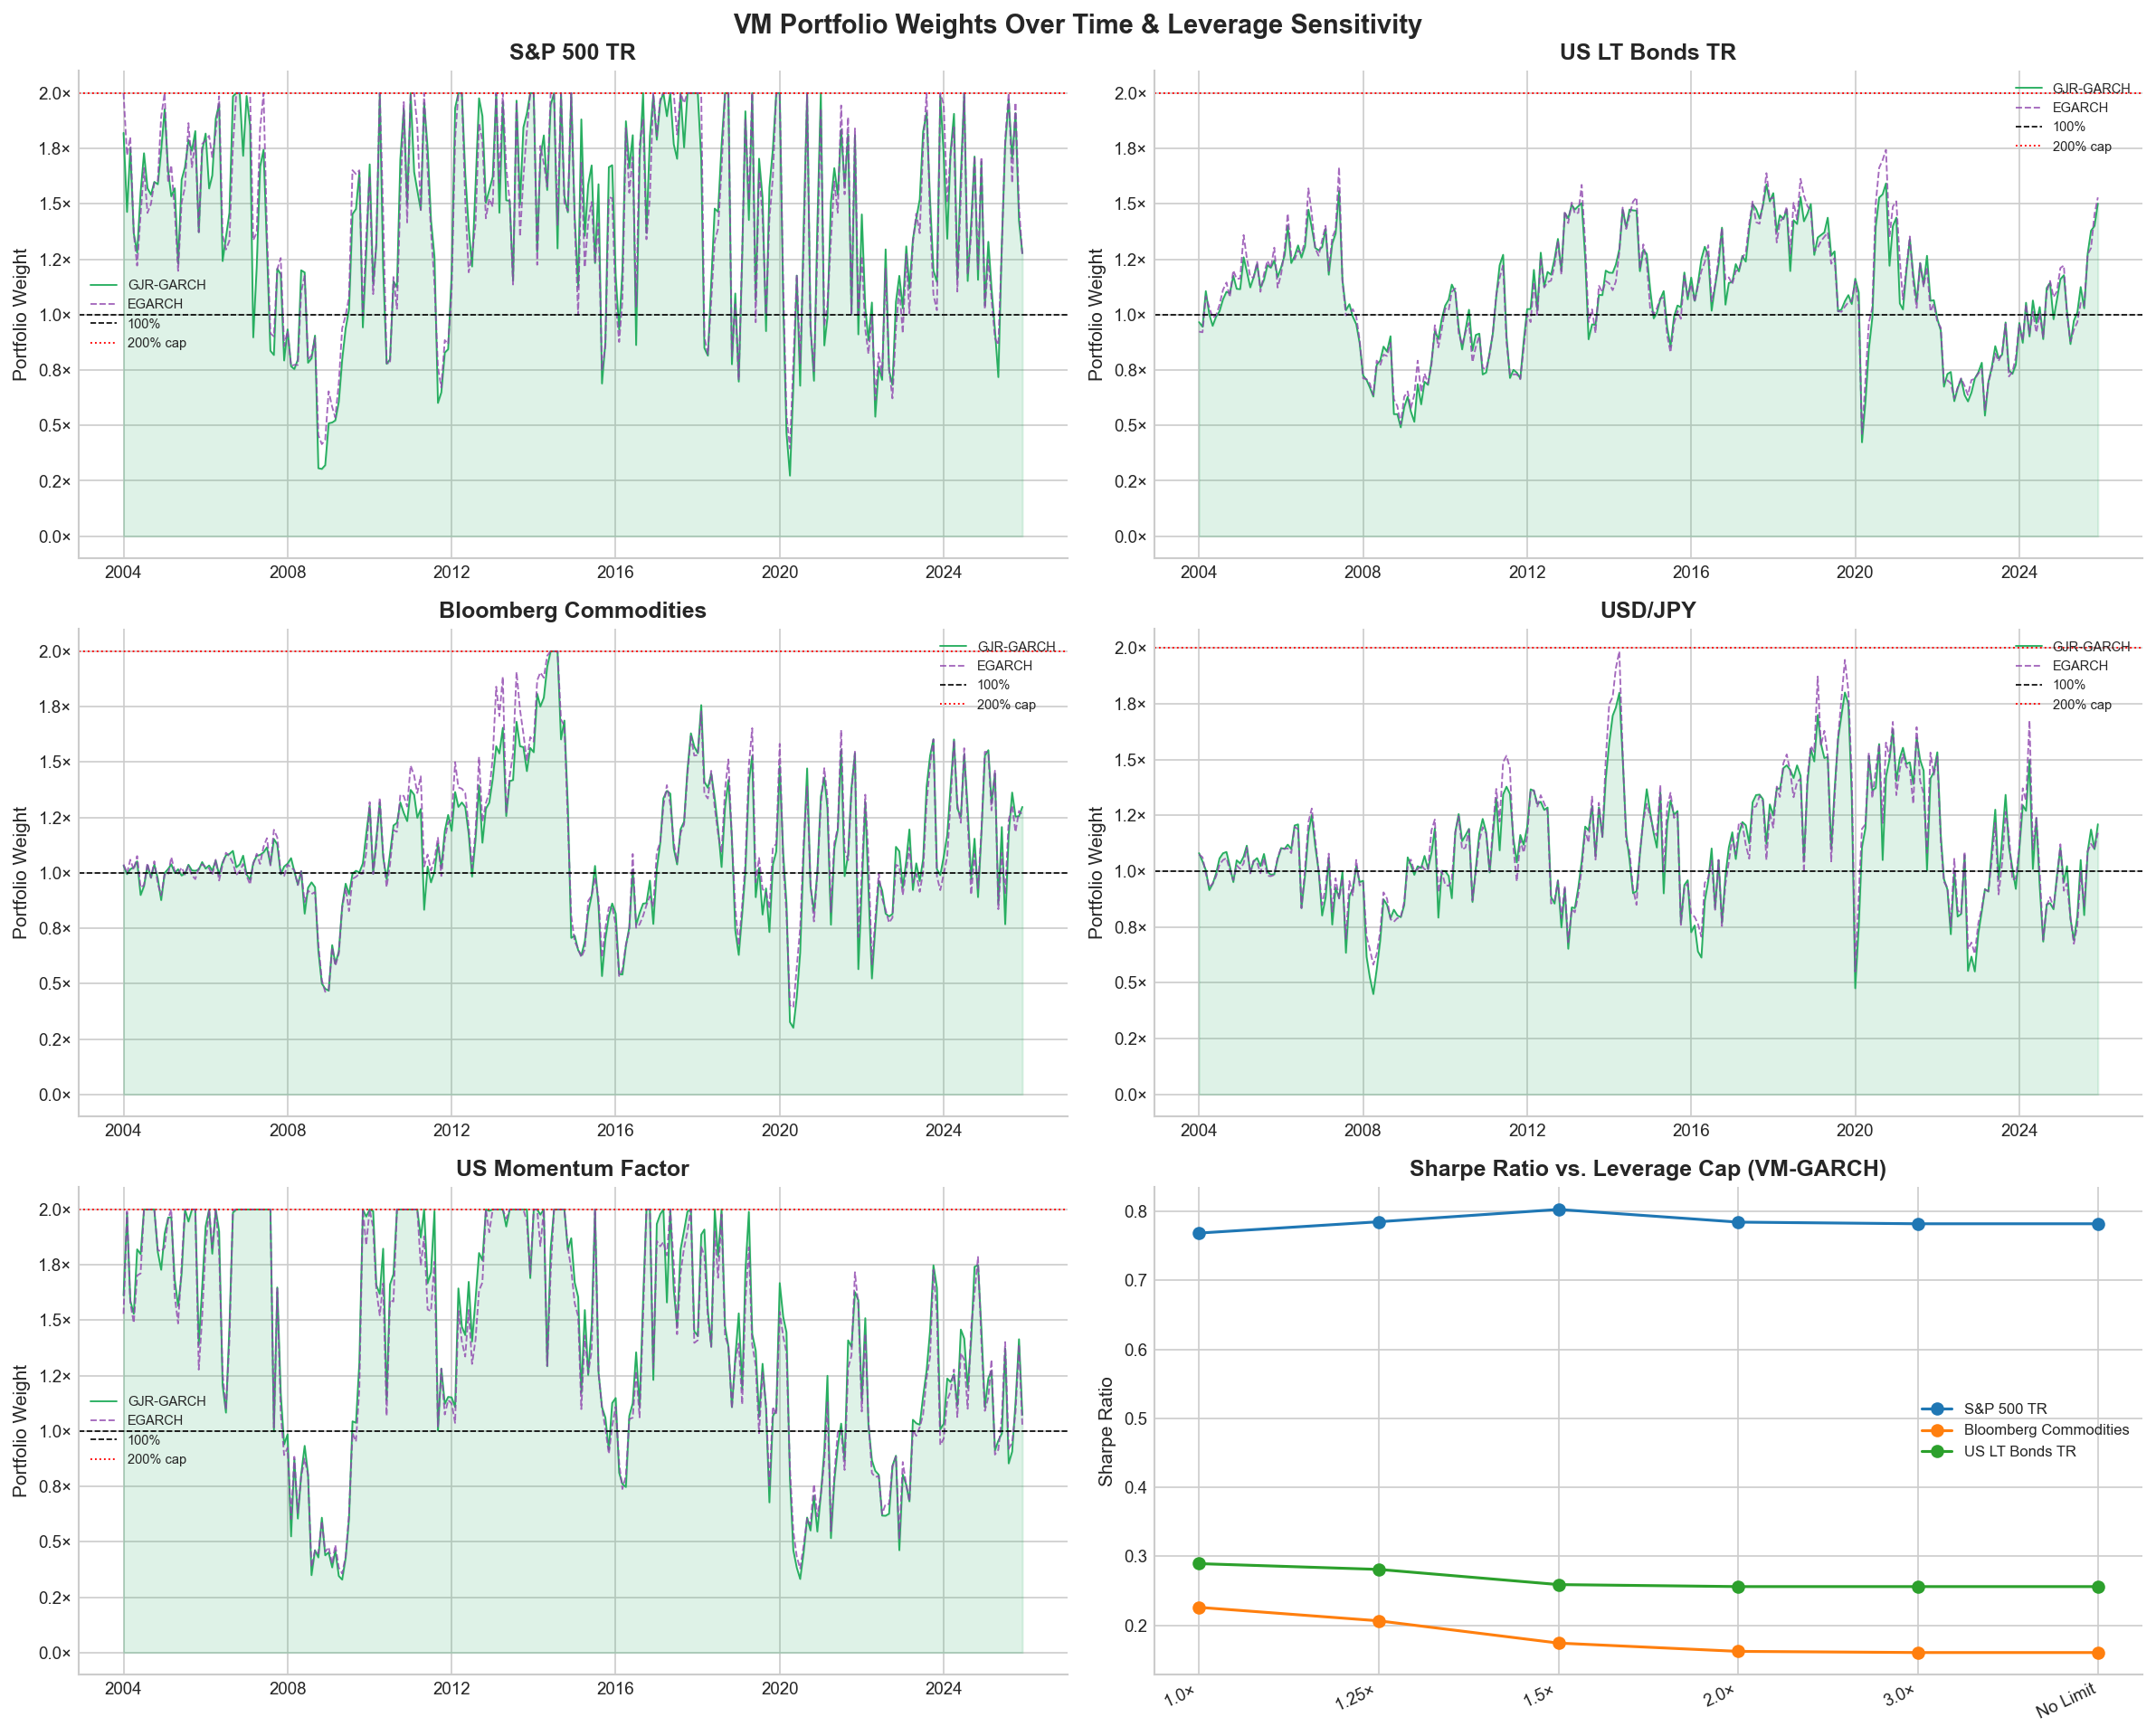
\includegraphics[width=0.9\textwidth]{fig_07_leverage.png}
  \caption{VM Portfolio Weights Over Time (GJR-GARCH and EGARCH, leverage cap = 200\%)
           and Sharpe Ratio Sensitivity to Leverage Constraints. For the S\&P 500 and the
           momentum factor, the cap binds frequently in low-volatility regimes
           (2014--2019, 2021--2023). For US long-term bonds, the cap rarely binds (the
           maximum weight is approximately 1.59). The Sharpe ratio for equities is
           maximised near a 1.5 leverage cap.}
  \label{fig:weights}
\end{figure}

\begin{figure}[H]
  \centering
  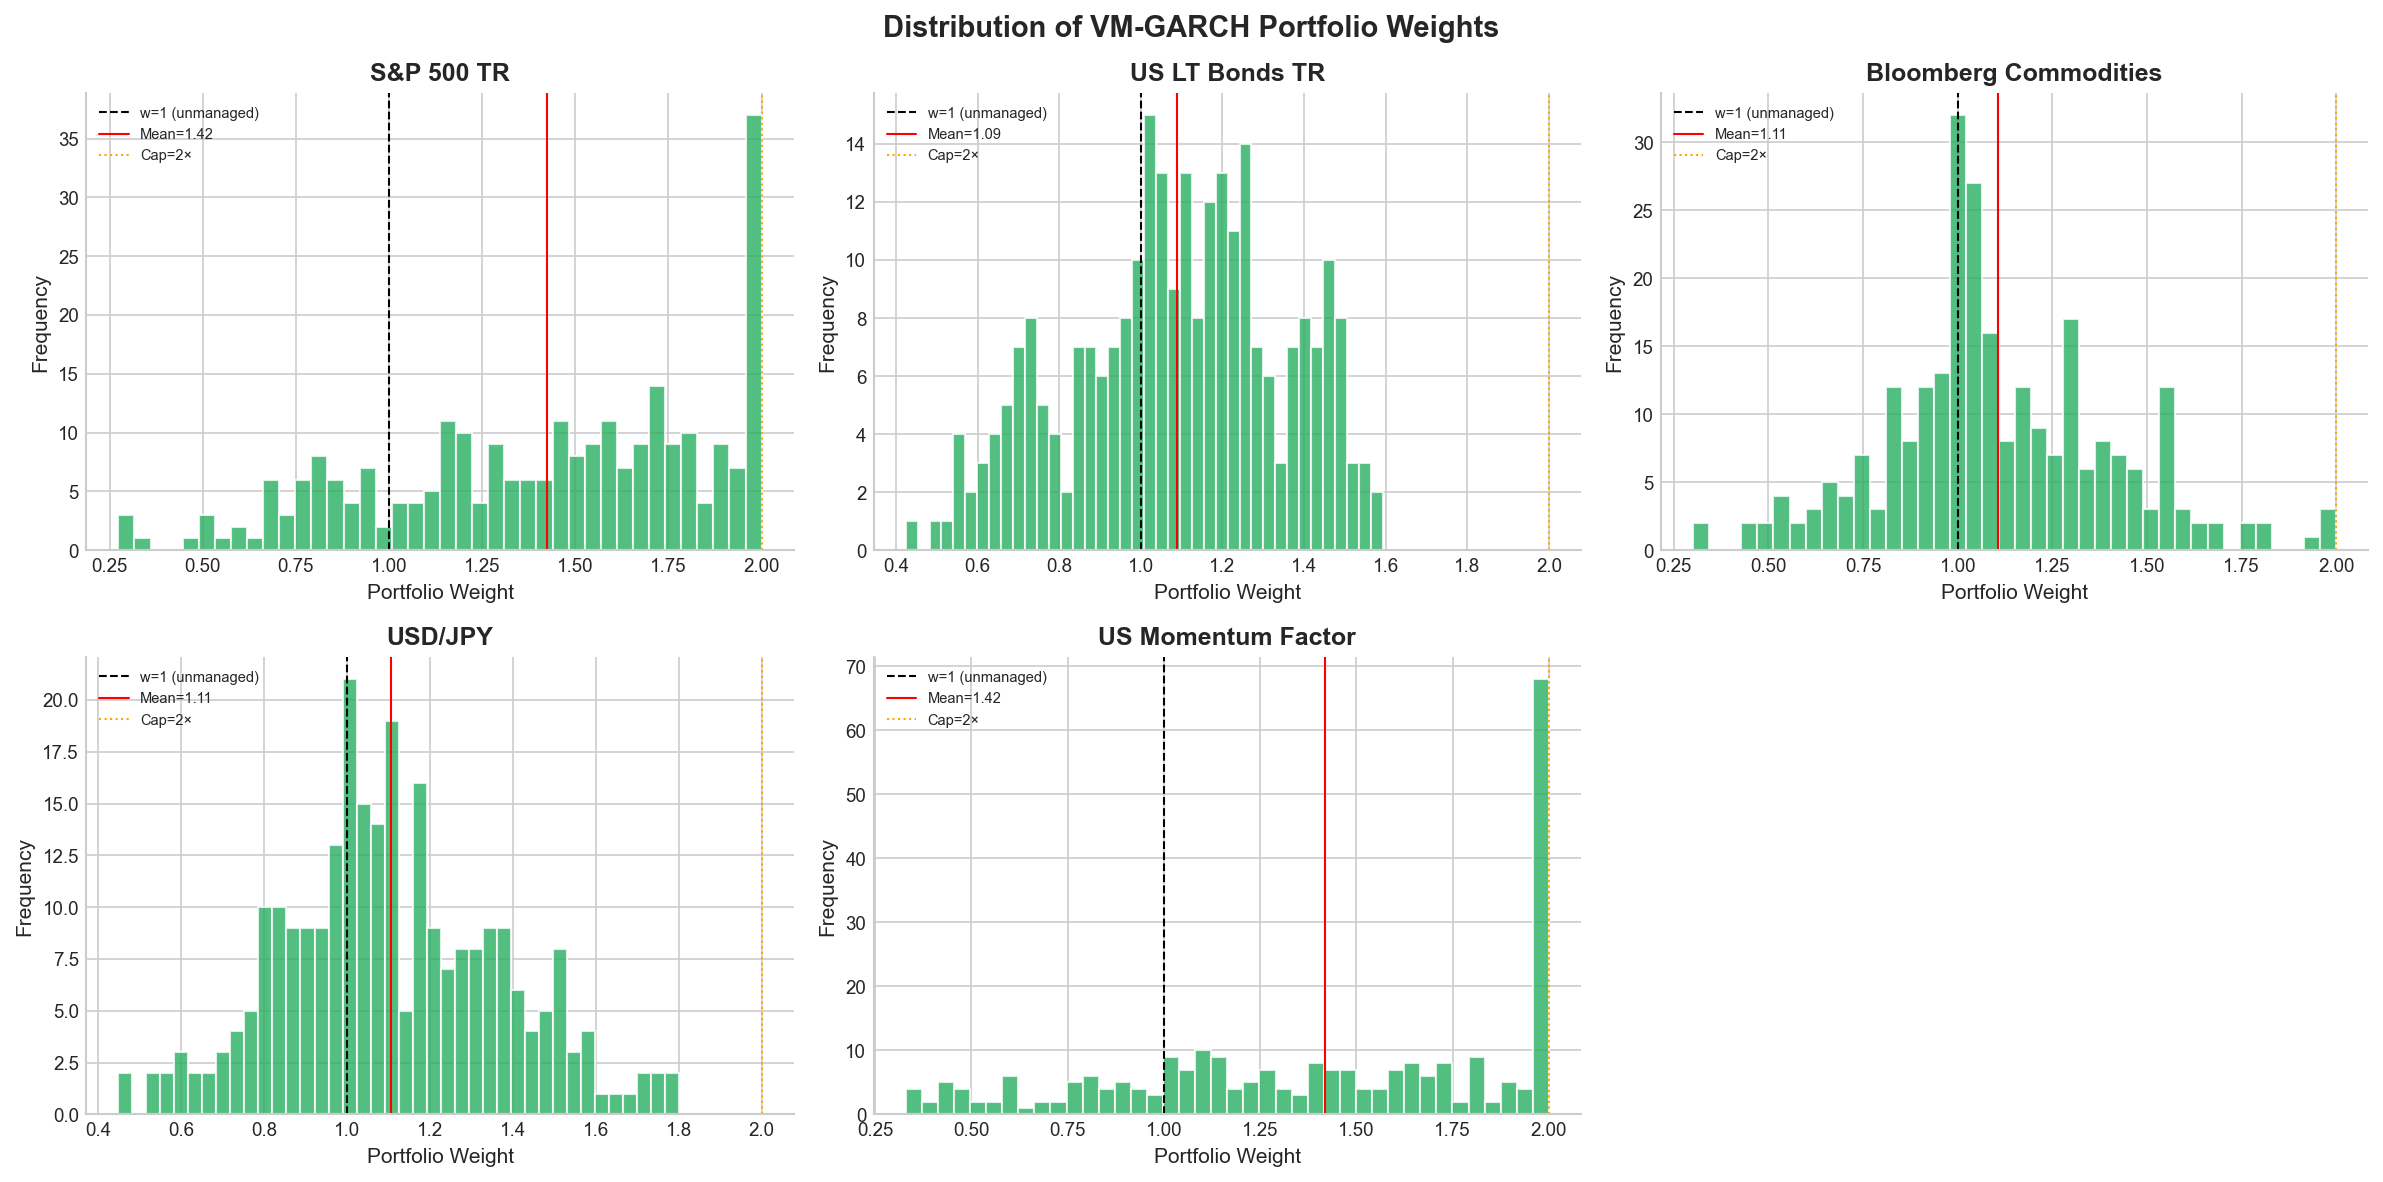
\includegraphics[width=0.85\textwidth]{fig_08_weight_distribution.png}
  \caption{Distribution of VM-GJR-GARCH Portfolio Weights across All Assets.
           The S\&P 500 and the momentum factor show strongly right-skewed weight
           distributions with a mass at the 2.0 leverage cap (mean weights 1.42 in both
           cases), reflecting persistent low-volatility regimes in the sample. US LT
           Bonds shows a near-uniform distribution (mean weight 1.09), consistent with a
           mean-reverting but continuous volatility process. Commodities cluster near
           weight 1.0 (mean 1.11) because the structurally high base volatility leaves
           little room to lever.}
  \label{fig:weight_dist}
\end{figure}
